% **************************************************************************************************************
% A Classic Thesis Style
% An Homage to The Elements of Typographic Style
%
% Copyright (C) 2015 André Miede http://www.miede.de
%
% If you like the style then I would appreciate a postcard. My address 
% can be found in the file ClassicThesis.pdf. A collection of the 
% postcards I received so far is available online at 
% http://postcards.miede.de
%
% License:
% This program is free software; you can redistribute it and/or modify
% it under the terms of the GNU General Public License as published by
% the Free Software Foundation; either version 2 of the License, or
% (at your option) any later version.
%
% This program is distributed in the hope that it will be useful,
% but WITHOUT ANY WARRANTY; without even the implied warranty of
% MERCHANTABILITY or FITNESS FOR A PARTICULAR PURPOSE.  See the
% GNU General Public License for more details.
%
% You should have received a copy of the GNU General Public License
% along with this program; see the file COPYING.  If not, write to
% the Free Software Foundation, Inc., 59 Temple Place - Suite 330,
% Boston, MA 02111-1307, USA.
%
% **************************************************************************************************************
% arara: pdflatex
% arara: bibtex
% arara: bibtex: { files: [ JDHV ] }
% arara: pdflatex
% arara: pdflatex
\RequirePackage{fix-cm} % fix some latex issues see: http://texdoc.net/texmf-dist/doc/latex/base/fixltx2e.pdf
\documentclass[ oneside,openright,titlepage,numbers=noenddot,headinclude,%1headlines,% letterpaper a4paper
                footinclude=false,cleardoublepage=empty,abstractoff, % <---
                % obsolete, remove (todo)
                BCOR=5mm,paper=a4,fontsize=11pt,%11pt,a4paper,%
                ngerman,american,%
                ]{scrreprt}

%********************************************************************
% Note: Make all your adjustments in here
%*******************************************************
% ****************************************************************************************************
% classicthesis-config.tex 
% formerly known as loadpackages.sty, classicthesis-ldpkg.sty, and classicthesis-preamble.sty 
% Use it at the beginning of your ClassicThesis.tex, or as a LaTeX Preamble 
% in your ClassicThesis.{tex,lyx} with % ****************************************************************************************************
% classicthesis-config.tex 
% formerly known as loadpackages.sty, classicthesis-ldpkg.sty, and classicthesis-preamble.sty 
% Use it at the beginning of your ClassicThesis.tex, or as a LaTeX Preamble 
% in your ClassicThesis.{tex,lyx} with % ****************************************************************************************************
% classicthesis-config.tex 
% formerly known as loadpackages.sty, classicthesis-ldpkg.sty, and classicthesis-preamble.sty 
% Use it at the beginning of your ClassicThesis.tex, or as a LaTeX Preamble 
% in your ClassicThesis.{tex,lyx} with \input{classicthesis-config}
% ****************************************************************************************************  
% If you like the classicthesis, then I would appreciate a postcard. 
% My address can be found in the file ClassicThesis.pdf. A collection 
% of the postcards I received so far is available online at 
% http://postcards.miede.de
% ****************************************************************************************************
\usepackage{color}
\usepackage{soul}
\usepackage{paralist}
\usepackage{makecell}
\usepackage[ruled,vlined,linesnumbered]{algorithm2e}
\renewcommand{\algorithmcfname}{Algorithm}
\usepackage{pdflscape}
% \usepackage[resetlabels,labeled]{multibib}
% \newcites{JDHV}{References2}
% ****************************************************************************************************
% 0. Set the encoding of your files. UTF-8 is the only sensible encoding nowadays. If you can't read
% äöüßáéçèê∂åëæƒÏ€ then change the encoding setting in your editor, not the line below. If your editor
% does not support utf8 use another editor!
% ****************************************************************************************************
\PassOptionsToPackage{utf8}{inputenc}
	\usepackage{inputenc}
	
% ****************************************************************************************************
% 1. Configure classicthesis for your needs here, e.g., remove "drafting" below 
% in order to deactivate the time-stamp on the pages
% ****************************************************************************************************
\PassOptionsToPackage{eulerchapternumbers,listings,drafting,%
					 pdfspacing,%floatperchapter,%linedheaders,%
					 subfig,beramono,eulermath,parts,dottedtoc}{classicthesis}                                        
% ********************************************************************
% Available options for classicthesis.sty 
% (see ClassicThesis.pdf for more information):
% drafting
% parts nochapters linedheaders
% eulerchapternumbers beramono eulermath pdfspacing minionprospacing
% tocaligned dottedtoc manychapters
% listings floatperchapter subfig
% ********************************************************************


% ****************************************************************************************************
% 2. Personal data and user ad-hoc commands
% ****************************************************************************************************
\newcommand{\myTitle}{Word-Metric-based Greedy Routing\break for Cayley Graphs\xspace}
\newcommand{\mySubtitle}{An Homage to The Elements of Typographic Style\xspace}
\newcommand{\myDegree}{\textit{Doctoral Thesis}\xspace}
\newcommand{\myName}{Daniela Aguirre Guerrero\xspace}
\newcommand{\myProf}{Put name here\xspace}
\newcommand{\myOtherProf}{Put name here\xspace}
\newcommand{\mySupervisor}{Dr. Pere Vilà Talleda\xspace}
\newcommand{\myOtherSupervisor}{Dr. Lluís Fàbrega Soler\xspace}
\newcommand{\myFaculty}{Put data here\xspace}
\newcommand{\myDepartment}{Put data here\xspace}
\newcommand{\myUni}{Put data here\xspace}
\newcommand{\myLocation}{Saarbrücken\xspace}
\newcommand{\myTime}{2018\xspace}
\newcommand{\myVersion}{version 4.2\xspace}
% ********************************************************************
% Setup, finetuning, and useful commands
% ********************************************************************
\newcounter{dummy} % necessary for correct hyperlinks (to index, bib, etc.)
\newlength{\abcd} % for ab..z string length calculation
\providecommand{\mLyX}{L\kern-.1667em\lower.25em\hbox{Y}\kern-.125emX\@}
\newcommand{\ie}{i.e.,~}
\newcommand{\Ie}{I.\,e.}
\newcommand{\eg}{e.g.,~}
\newcommand{\Eg}{E.\,g.}
\newcommand{\etal}{et~al.~}
% ****************************************************************************************************


% ****************************************************************************************************
% 3. Loading some handy packages
% ****************************************************************************************************
% ******************************************************************** 
% Packages with options that might require adjustments
% ******************************************************************** 
%To enumerate My Publications
\usepackage[shortlabels]{enumitem}
%\PassOptionsToPackage{ngerman,american}{babel}   % change this to your language(s)
% Spanish languages need extra options in order to work with this template
%\PassOptionsToPackage{spanish,es-lcroman}{babel}
	\usepackage{babel}                  

\usepackage{csquotes}
\PassOptionsToPackage{%
    %backend=biber, %instead of bibtex
	backend=bibtex8,bibencoding=ascii,%
	language=auto,%
	style=numeric-comp,% authoryear, numeric-comp
    %style=authoryear-comp, % Author 1999, 2010
    %bibstyle=authoryear,dashed=false, % dashed: substitute rep. author with ---
    sorting=nyt, % name, year, title
    maxbibnames=10, % default: 3, et al.
    %backref=true,%
    natbib=true % natbib compatibility mode (\citep and \citet still work)
}{biblatex}
    \usepackage{biblatex}
    
% \usepackage[giveninits=true, isbn=false, url=false, doi=false,
% style=ieee, defernumbers=true, sorting=ydnt, bibstyle=ieee,
% maxnames=5, backend=biber]{biblatex}
    



\PassOptionsToPackage{fleqn}{amsmath}       % math environments and more by the AMS 
    \usepackage{amsmath}

% ******************************************************************** 
% General useful packages
% ******************************************************************** 
\PassOptionsToPackage{T1}{fontenc} % T2A for cyrillics
    \usepackage{fontenc}     
\usepackage{textcomp} % fix warning with missing font shapes
\usepackage{scrhack} % fix warnings when using KOMA with listings package          
\usepackage{xspace} % to get the spacing after macros right  
\usepackage{mparhack} % get marginpar right
\usepackage{fixltx2e} % fixes some LaTeX stuff --> since 2015 in the LaTeX kernel (see below)
%\usepackage[latest]{latexrelease} % will be used once available in more distributions (ISSUE #107)
\PassOptionsToPackage{printonlyused,smaller}{acronym} 
    \usepackage{acronym} % nice macros for handling all acronyms in the thesis
    %\renewcommand{\bflabel}[1]{{#1}\hfill} % fix the list of acronyms --> no longer working
    %\renewcommand*{\acsfont}[1]{\textsc{#1}} 
    \renewcommand*{\aclabelfont}[1]{\acsfont{#1}}
% ****************************************************************************************************


% ****************************************************************************************************
% 4. Setup floats: tables, (sub)figures, and captions
% ****************************************************************************************************
\usepackage{tabularx} % better tables
    \setlength{\extrarowheight}{3pt} % increase table row height
\newcommand{\tableheadline}[1]{\multicolumn{1}{c}{\spacedlowsmallcaps{#1}}}
\newcommand{\myfloatalign}{\centering} % to be used with each float for alignment
\usepackage{caption}
% Thanks to cgnieder and Claus Lahiri
% http://tex.stackexchange.com/questions/69349/spacedlowsmallcaps-in-caption-label
% [REMOVED DUE TO OTHER PROBLEMS, SEE ISSUE #82]    
%\DeclareCaptionLabelFormat{smallcaps}{\bothIfFirst{#1}{~}\MakeTextLowercase{\textsc{#2}}}
%\captionsetup{font=small,labelformat=smallcaps} % format=hang,
\captionsetup{font=small} % format=hang,
\usepackage{subfig}  
% ****************************************************************************************************


% ****************************************************************************************************
% 5. Setup code listings
% ****************************************************************************************************
\usepackage{listings} 
%\lstset{emph={trueIndex,root},emphstyle=\color{BlueViolet}}%\underbar} % for special keywords
\lstset{language=[LaTeX]Tex,%C++,
    morekeywords={PassOptionsToPackage,selectlanguage},
    keywordstyle=\color{RoyalBlue},%\bfseries,
    basicstyle=\small\ttfamily,
    %identifierstyle=\color{NavyBlue},
    commentstyle=\color{Green}\ttfamily,
    stringstyle=\rmfamily,
    numbers=none,%left,%
    numberstyle=\scriptsize,%\tiny
    stepnumber=5,
    numbersep=8pt,
    showstringspaces=false,
    breaklines=true,
    %frameround=ftff,
    %frame=single,
    belowcaptionskip=.75\baselineskip
    %frame=L
} 
% ****************************************************************************************************             


% ****************************************************************************************************
% 6. PDFLaTeX, hyperreferences and citation backreferences
% ****************************************************************************************************
% ********************************************************************
% Using PDFLaTeX
% ********************************************************************
\PassOptionsToPackage{pdftex,hyperfootnotes=false,pdfpagelabels}{hyperref}
    \usepackage{hyperref}  % backref linktocpage pagebackref
\pdfcompresslevel=9
\pdfadjustspacing=1 
\PassOptionsToPackage{pdftex}{graphicx}
    \usepackage{graphicx} 
 

% ********************************************************************
% Hyperreferences
% ********************************************************************
\hypersetup{%
    %draft, % = no hyperlinking at all (useful in b/w printouts)
    colorlinks=true, linktocpage=true, pdfstartpage=3, pdfstartview=FitV,%
    % uncomment the following line if you want to have black links (e.g., for printing)
    %colorlinks=false, linktocpage=false, pdfstartpage=3, pdfstartview=FitV, pdfborder={0 0 0},%
    breaklinks=true, pdfpagemode=UseNone, pageanchor=true, pdfpagemode=UseOutlines,%
    plainpages=false, bookmarksnumbered, bookmarksopen=true, bookmarksopenlevel=1,%
    hypertexnames=true, pdfhighlight=/O,%nesting=true,%frenchlinks,%
    urlcolor=webbrown, linkcolor=RoyalBlue, citecolor=webgreen, %pagecolor=RoyalBlue,%
    %urlcolor=Black, linkcolor=Black, citecolor=Black, %pagecolor=Black,%
    pdftitle={\myTitle},%
    pdfauthor={\textcopyright\ \myName, \myUni, \myFaculty},%
    pdfsubject={},%
    pdfkeywords={},%
    pdfcreator={pdfLaTeX},%
    pdfproducer={LaTeX with hyperref and classicthesis}%
}   

% ********************************************************************
% Setup autoreferences
% ********************************************************************
% There are some issues regarding autorefnames
% http://www.ureader.de/msg/136221647.aspx
% http://www.tex.ac.uk/cgi-bin/texfaq2html?label=latexwords
% you have to redefine the makros for the 
% language you use, e.g., american, ngerman
% (as chosen when loading babel/AtBeginDocument)
% ********************************************************************
\makeatletter
\@ifpackageloaded{babel}%
    {%
       \addto\extrasamerican{%
			\renewcommand*{\figureautorefname}{Figure}%
			\renewcommand*{\tableautorefname}{Table}%
			\renewcommand*{\partautorefname}{Part}%
			\renewcommand*{\chapterautorefname}{Chapter}%
			\renewcommand*{\sectionautorefname}{Section}%
			\renewcommand*{\subsectionautorefname}{Section}%
			\renewcommand*{\subsubsectionautorefname}{Section}%     
                }%
       \addto\extrasngerman{% 
			\renewcommand*{\paragraphautorefname}{Absatz}%
			\renewcommand*{\subparagraphautorefname}{Unterabsatz}%
			\renewcommand*{\footnoteautorefname}{Fu\"snote}%
			\renewcommand*{\FancyVerbLineautorefname}{Zeile}%
			\renewcommand*{\theoremautorefname}{Theorem}%
			\renewcommand*{\appendixautorefname}{Anhang}%
			\renewcommand*{\equationautorefname}{Gleichung}%        
			\renewcommand*{\itemautorefname}{Punkt}%
                }%  
            % Fix to getting autorefs for subfigures right (thanks to Belinda Vogt for changing the definition)
            \providecommand{\subfigureautorefname}{\figureautorefname}%             
    }{\relax}
\makeatother


% ****************************************************************************************************
% 7. Last calls before the bar closes
% ****************************************************************************************************
% ********************************************************************
% Development Stuff
% ********************************************************************
\listfiles
%\PassOptionsToPackage{l2tabu,orthodox,abort}{nag}
%   \usepackage{nag}
%\PassOptionsToPackage{warning, all}{onlyamsmath}
%   \usepackage{onlyamsmath}

% ********************************************************************
% Last, but not least...
% ********************************************************************
\usepackage{classicthesis} 
% ****************************************************************************************************


% ****************************************************************************************************
% 8. Further adjustments (experimental)
% ****************************************************************************************************
% ********************************************************************
% Changing the text area
% ********************************************************************
%\linespread{1.05} % a bit more for Palatino
\areaset[current]{360pt}{750pt} % 686 (factor 2.2) + 33 head + 42 head \the\footskip
\setlength{\marginparwidth}{7em}%
\setlength{\marginparsep}{2em}%

\usepackage{etoolbox}

\makeatletter
\patchcmd{\ttlh@hang}{\parindent\z@}{\parindent\z@\leavevmode}{}{}
\patchcmd{\ttlh@hang}{\noindent}{}{}{}
\makeatother

% ********************************************************************
% Using different fonts
% ********************************************************************
%\usepackage[oldstylenums]{kpfonts} % oldstyle notextcomp
%\usepackage[osf]{libertine}
%\usepackage[light,condensed,math]{iwona}
%\renewcommand{\sfdefault}{iwona}
%\usepackage{lmodern} % <-- no osf support :-(
%\usepackage{cfr-lm} % 
%\usepackage[urw-garamond]{mathdesign} <-- no osf support :-(
%\usepackage[default,osfigures]{opensans} % scale=0.95 
%\usepackage[sfdefault]{FiraSans}
% ****************************************************************************************************

% ****************************************************************************************************  
% If you like the classicthesis, then I would appreciate a postcard. 
% My address can be found in the file ClassicThesis.pdf. A collection 
% of the postcards I received so far is available online at 
% http://postcards.miede.de
% ****************************************************************************************************
\usepackage{color}
\usepackage{soul}
\usepackage{paralist}
\usepackage{makecell}
\usepackage[ruled,vlined,linesnumbered]{algorithm2e}
\renewcommand{\algorithmcfname}{Algorithm}
\usepackage{pdflscape}
% \usepackage[resetlabels,labeled]{multibib}
% \newcites{JDHV}{References2}
% ****************************************************************************************************
% 0. Set the encoding of your files. UTF-8 is the only sensible encoding nowadays. If you can't read
% äöüßáéçèê∂åëæƒÏ€ then change the encoding setting in your editor, not the line below. If your editor
% does not support utf8 use another editor!
% ****************************************************************************************************
\PassOptionsToPackage{utf8}{inputenc}
	\usepackage{inputenc}
	
% ****************************************************************************************************
% 1. Configure classicthesis for your needs here, e.g., remove "drafting" below 
% in order to deactivate the time-stamp on the pages
% ****************************************************************************************************
\PassOptionsToPackage{eulerchapternumbers,listings,drafting,%
					 pdfspacing,%floatperchapter,%linedheaders,%
					 subfig,beramono,eulermath,parts,dottedtoc}{classicthesis}                                        
% ********************************************************************
% Available options for classicthesis.sty 
% (see ClassicThesis.pdf for more information):
% drafting
% parts nochapters linedheaders
% eulerchapternumbers beramono eulermath pdfspacing minionprospacing
% tocaligned dottedtoc manychapters
% listings floatperchapter subfig
% ********************************************************************


% ****************************************************************************************************
% 2. Personal data and user ad-hoc commands
% ****************************************************************************************************
\newcommand{\myTitle}{Word-Metric-based Greedy Routing\break for Cayley Graphs\xspace}
\newcommand{\mySubtitle}{An Homage to The Elements of Typographic Style\xspace}
\newcommand{\myDegree}{\textit{Doctoral Thesis}\xspace}
\newcommand{\myName}{Daniela Aguirre Guerrero\xspace}
\newcommand{\myProf}{Put name here\xspace}
\newcommand{\myOtherProf}{Put name here\xspace}
\newcommand{\mySupervisor}{Dr. Pere Vilà Talleda\xspace}
\newcommand{\myOtherSupervisor}{Dr. Lluís Fàbrega Soler\xspace}
\newcommand{\myFaculty}{Put data here\xspace}
\newcommand{\myDepartment}{Put data here\xspace}
\newcommand{\myUni}{Put data here\xspace}
\newcommand{\myLocation}{Saarbrücken\xspace}
\newcommand{\myTime}{2018\xspace}
\newcommand{\myVersion}{version 4.2\xspace}
% ********************************************************************
% Setup, finetuning, and useful commands
% ********************************************************************
\newcounter{dummy} % necessary for correct hyperlinks (to index, bib, etc.)
\newlength{\abcd} % for ab..z string length calculation
\providecommand{\mLyX}{L\kern-.1667em\lower.25em\hbox{Y}\kern-.125emX\@}
\newcommand{\ie}{i.e.,~}
\newcommand{\Ie}{I.\,e.}
\newcommand{\eg}{e.g.,~}
\newcommand{\Eg}{E.\,g.}
\newcommand{\etal}{et~al.~}
% ****************************************************************************************************


% ****************************************************************************************************
% 3. Loading some handy packages
% ****************************************************************************************************
% ******************************************************************** 
% Packages with options that might require adjustments
% ******************************************************************** 
%To enumerate My Publications
\usepackage[shortlabels]{enumitem}
%\PassOptionsToPackage{ngerman,american}{babel}   % change this to your language(s)
% Spanish languages need extra options in order to work with this template
%\PassOptionsToPackage{spanish,es-lcroman}{babel}
	\usepackage{babel}                  

\usepackage{csquotes}
\PassOptionsToPackage{%
    %backend=biber, %instead of bibtex
	backend=bibtex8,bibencoding=ascii,%
	language=auto,%
	style=numeric-comp,% authoryear, numeric-comp
    %style=authoryear-comp, % Author 1999, 2010
    %bibstyle=authoryear,dashed=false, % dashed: substitute rep. author with ---
    sorting=nyt, % name, year, title
    maxbibnames=10, % default: 3, et al.
    %backref=true,%
    natbib=true % natbib compatibility mode (\citep and \citet still work)
}{biblatex}
    \usepackage{biblatex}
    
% \usepackage[giveninits=true, isbn=false, url=false, doi=false,
% style=ieee, defernumbers=true, sorting=ydnt, bibstyle=ieee,
% maxnames=5, backend=biber]{biblatex}
    



\PassOptionsToPackage{fleqn}{amsmath}       % math environments and more by the AMS 
    \usepackage{amsmath}

% ******************************************************************** 
% General useful packages
% ******************************************************************** 
\PassOptionsToPackage{T1}{fontenc} % T2A for cyrillics
    \usepackage{fontenc}     
\usepackage{textcomp} % fix warning with missing font shapes
\usepackage{scrhack} % fix warnings when using KOMA with listings package          
\usepackage{xspace} % to get the spacing after macros right  
\usepackage{mparhack} % get marginpar right
\usepackage{fixltx2e} % fixes some LaTeX stuff --> since 2015 in the LaTeX kernel (see below)
%\usepackage[latest]{latexrelease} % will be used once available in more distributions (ISSUE #107)
\PassOptionsToPackage{printonlyused,smaller}{acronym} 
    \usepackage{acronym} % nice macros for handling all acronyms in the thesis
    %\renewcommand{\bflabel}[1]{{#1}\hfill} % fix the list of acronyms --> no longer working
    %\renewcommand*{\acsfont}[1]{\textsc{#1}} 
    \renewcommand*{\aclabelfont}[1]{\acsfont{#1}}
% ****************************************************************************************************


% ****************************************************************************************************
% 4. Setup floats: tables, (sub)figures, and captions
% ****************************************************************************************************
\usepackage{tabularx} % better tables
    \setlength{\extrarowheight}{3pt} % increase table row height
\newcommand{\tableheadline}[1]{\multicolumn{1}{c}{\spacedlowsmallcaps{#1}}}
\newcommand{\myfloatalign}{\centering} % to be used with each float for alignment
\usepackage{caption}
% Thanks to cgnieder and Claus Lahiri
% http://tex.stackexchange.com/questions/69349/spacedlowsmallcaps-in-caption-label
% [REMOVED DUE TO OTHER PROBLEMS, SEE ISSUE #82]    
%\DeclareCaptionLabelFormat{smallcaps}{\bothIfFirst{#1}{~}\MakeTextLowercase{\textsc{#2}}}
%\captionsetup{font=small,labelformat=smallcaps} % format=hang,
\captionsetup{font=small} % format=hang,
\usepackage{subfig}  
% ****************************************************************************************************


% ****************************************************************************************************
% 5. Setup code listings
% ****************************************************************************************************
\usepackage{listings} 
%\lstset{emph={trueIndex,root},emphstyle=\color{BlueViolet}}%\underbar} % for special keywords
\lstset{language=[LaTeX]Tex,%C++,
    morekeywords={PassOptionsToPackage,selectlanguage},
    keywordstyle=\color{RoyalBlue},%\bfseries,
    basicstyle=\small\ttfamily,
    %identifierstyle=\color{NavyBlue},
    commentstyle=\color{Green}\ttfamily,
    stringstyle=\rmfamily,
    numbers=none,%left,%
    numberstyle=\scriptsize,%\tiny
    stepnumber=5,
    numbersep=8pt,
    showstringspaces=false,
    breaklines=true,
    %frameround=ftff,
    %frame=single,
    belowcaptionskip=.75\baselineskip
    %frame=L
} 
% ****************************************************************************************************             


% ****************************************************************************************************
% 6. PDFLaTeX, hyperreferences and citation backreferences
% ****************************************************************************************************
% ********************************************************************
% Using PDFLaTeX
% ********************************************************************
\PassOptionsToPackage{pdftex,hyperfootnotes=false,pdfpagelabels}{hyperref}
    \usepackage{hyperref}  % backref linktocpage pagebackref
\pdfcompresslevel=9
\pdfadjustspacing=1 
\PassOptionsToPackage{pdftex}{graphicx}
    \usepackage{graphicx} 
 

% ********************************************************************
% Hyperreferences
% ********************************************************************
\hypersetup{%
    %draft, % = no hyperlinking at all (useful in b/w printouts)
    colorlinks=true, linktocpage=true, pdfstartpage=3, pdfstartview=FitV,%
    % uncomment the following line if you want to have black links (e.g., for printing)
    %colorlinks=false, linktocpage=false, pdfstartpage=3, pdfstartview=FitV, pdfborder={0 0 0},%
    breaklinks=true, pdfpagemode=UseNone, pageanchor=true, pdfpagemode=UseOutlines,%
    plainpages=false, bookmarksnumbered, bookmarksopen=true, bookmarksopenlevel=1,%
    hypertexnames=true, pdfhighlight=/O,%nesting=true,%frenchlinks,%
    urlcolor=webbrown, linkcolor=RoyalBlue, citecolor=webgreen, %pagecolor=RoyalBlue,%
    %urlcolor=Black, linkcolor=Black, citecolor=Black, %pagecolor=Black,%
    pdftitle={\myTitle},%
    pdfauthor={\textcopyright\ \myName, \myUni, \myFaculty},%
    pdfsubject={},%
    pdfkeywords={},%
    pdfcreator={pdfLaTeX},%
    pdfproducer={LaTeX with hyperref and classicthesis}%
}   

% ********************************************************************
% Setup autoreferences
% ********************************************************************
% There are some issues regarding autorefnames
% http://www.ureader.de/msg/136221647.aspx
% http://www.tex.ac.uk/cgi-bin/texfaq2html?label=latexwords
% you have to redefine the makros for the 
% language you use, e.g., american, ngerman
% (as chosen when loading babel/AtBeginDocument)
% ********************************************************************
\makeatletter
\@ifpackageloaded{babel}%
    {%
       \addto\extrasamerican{%
			\renewcommand*{\figureautorefname}{Figure}%
			\renewcommand*{\tableautorefname}{Table}%
			\renewcommand*{\partautorefname}{Part}%
			\renewcommand*{\chapterautorefname}{Chapter}%
			\renewcommand*{\sectionautorefname}{Section}%
			\renewcommand*{\subsectionautorefname}{Section}%
			\renewcommand*{\subsubsectionautorefname}{Section}%     
                }%
       \addto\extrasngerman{% 
			\renewcommand*{\paragraphautorefname}{Absatz}%
			\renewcommand*{\subparagraphautorefname}{Unterabsatz}%
			\renewcommand*{\footnoteautorefname}{Fu\"snote}%
			\renewcommand*{\FancyVerbLineautorefname}{Zeile}%
			\renewcommand*{\theoremautorefname}{Theorem}%
			\renewcommand*{\appendixautorefname}{Anhang}%
			\renewcommand*{\equationautorefname}{Gleichung}%        
			\renewcommand*{\itemautorefname}{Punkt}%
                }%  
            % Fix to getting autorefs for subfigures right (thanks to Belinda Vogt for changing the definition)
            \providecommand{\subfigureautorefname}{\figureautorefname}%             
    }{\relax}
\makeatother


% ****************************************************************************************************
% 7. Last calls before the bar closes
% ****************************************************************************************************
% ********************************************************************
% Development Stuff
% ********************************************************************
\listfiles
%\PassOptionsToPackage{l2tabu,orthodox,abort}{nag}
%   \usepackage{nag}
%\PassOptionsToPackage{warning, all}{onlyamsmath}
%   \usepackage{onlyamsmath}

% ********************************************************************
% Last, but not least...
% ********************************************************************
\usepackage{classicthesis} 
% ****************************************************************************************************


% ****************************************************************************************************
% 8. Further adjustments (experimental)
% ****************************************************************************************************
% ********************************************************************
% Changing the text area
% ********************************************************************
%\linespread{1.05} % a bit more for Palatino
\areaset[current]{360pt}{750pt} % 686 (factor 2.2) + 33 head + 42 head \the\footskip
\setlength{\marginparwidth}{7em}%
\setlength{\marginparsep}{2em}%

\usepackage{etoolbox}

\makeatletter
\patchcmd{\ttlh@hang}{\parindent\z@}{\parindent\z@\leavevmode}{}{}
\patchcmd{\ttlh@hang}{\noindent}{}{}{}
\makeatother

% ********************************************************************
% Using different fonts
% ********************************************************************
%\usepackage[oldstylenums]{kpfonts} % oldstyle notextcomp
%\usepackage[osf]{libertine}
%\usepackage[light,condensed,math]{iwona}
%\renewcommand{\sfdefault}{iwona}
%\usepackage{lmodern} % <-- no osf support :-(
%\usepackage{cfr-lm} % 
%\usepackage[urw-garamond]{mathdesign} <-- no osf support :-(
%\usepackage[default,osfigures]{opensans} % scale=0.95 
%\usepackage[sfdefault]{FiraSans}
% ****************************************************************************************************

% ****************************************************************************************************  
% If you like the classicthesis, then I would appreciate a postcard. 
% My address can be found in the file ClassicThesis.pdf. A collection 
% of the postcards I received so far is available online at 
% http://postcards.miede.de
% ****************************************************************************************************
\usepackage{color}
\usepackage{soul}
\usepackage{paralist}
\usepackage{makecell}
\usepackage[ruled,vlined,linesnumbered]{algorithm2e}
\renewcommand{\algorithmcfname}{Algorithm}
\usepackage{pdflscape}
% \usepackage[resetlabels,labeled]{multibib}
% \newcites{JDHV}{References2}
% ****************************************************************************************************
% 0. Set the encoding of your files. UTF-8 is the only sensible encoding nowadays. If you can't read
% äöüßáéçèê∂åëæƒÏ€ then change the encoding setting in your editor, not the line below. If your editor
% does not support utf8 use another editor!
% ****************************************************************************************************
\PassOptionsToPackage{utf8}{inputenc}
	\usepackage{inputenc}
	
% ****************************************************************************************************
% 1. Configure classicthesis for your needs here, e.g., remove "drafting" below 
% in order to deactivate the time-stamp on the pages
% ****************************************************************************************************
\PassOptionsToPackage{eulerchapternumbers,listings,drafting,%
					 pdfspacing,%floatperchapter,%linedheaders,%
					 subfig,beramono,eulermath,parts,dottedtoc}{classicthesis}                                        
% ********************************************************************
% Available options for classicthesis.sty 
% (see ClassicThesis.pdf for more information):
% drafting
% parts nochapters linedheaders
% eulerchapternumbers beramono eulermath pdfspacing minionprospacing
% tocaligned dottedtoc manychapters
% listings floatperchapter subfig
% ********************************************************************


% ****************************************************************************************************
% 2. Personal data and user ad-hoc commands
% ****************************************************************************************************
\newcommand{\myTitle}{Word-Metric-based Greedy Routing\break for Cayley Graphs\xspace}
\newcommand{\mySubtitle}{An Homage to The Elements of Typographic Style\xspace}
\newcommand{\myDegree}{\textit{Doctoral Thesis}\xspace}
\newcommand{\myName}{Daniela Aguirre Guerrero\xspace}
\newcommand{\myProf}{Put name here\xspace}
\newcommand{\myOtherProf}{Put name here\xspace}
\newcommand{\mySupervisor}{Dr. Pere Vilà Talleda\xspace}
\newcommand{\myOtherSupervisor}{Dr. Lluís Fàbrega Soler\xspace}
\newcommand{\myFaculty}{Put data here\xspace}
\newcommand{\myDepartment}{Put data here\xspace}
\newcommand{\myUni}{Put data here\xspace}
\newcommand{\myLocation}{Saarbrücken\xspace}
\newcommand{\myTime}{2018\xspace}
\newcommand{\myVersion}{version 4.2\xspace}
% ********************************************************************
% Setup, finetuning, and useful commands
% ********************************************************************
\newcounter{dummy} % necessary for correct hyperlinks (to index, bib, etc.)
\newlength{\abcd} % for ab..z string length calculation
\providecommand{\mLyX}{L\kern-.1667em\lower.25em\hbox{Y}\kern-.125emX\@}
\newcommand{\ie}{i.e.,~}
\newcommand{\Ie}{I.\,e.}
\newcommand{\eg}{e.g.,~}
\newcommand{\Eg}{E.\,g.}
\newcommand{\etal}{et~al.~}
% ****************************************************************************************************


% ****************************************************************************************************
% 3. Loading some handy packages
% ****************************************************************************************************
% ******************************************************************** 
% Packages with options that might require adjustments
% ******************************************************************** 
%To enumerate My Publications
\usepackage[shortlabels]{enumitem}
%\PassOptionsToPackage{ngerman,american}{babel}   % change this to your language(s)
% Spanish languages need extra options in order to work with this template
%\PassOptionsToPackage{spanish,es-lcroman}{babel}
	\usepackage{babel}                  

\usepackage{csquotes}
\PassOptionsToPackage{%
    %backend=biber, %instead of bibtex
	backend=bibtex8,bibencoding=ascii,%
	language=auto,%
	style=numeric-comp,% authoryear, numeric-comp
    %style=authoryear-comp, % Author 1999, 2010
    %bibstyle=authoryear,dashed=false, % dashed: substitute rep. author with ---
    sorting=nyt, % name, year, title
    maxbibnames=10, % default: 3, et al.
    %backref=true,%
    natbib=true % natbib compatibility mode (\citep and \citet still work)
}{biblatex}
    \usepackage{biblatex}
    
% \usepackage[giveninits=true, isbn=false, url=false, doi=false,
% style=ieee, defernumbers=true, sorting=ydnt, bibstyle=ieee,
% maxnames=5, backend=biber]{biblatex}
    



\PassOptionsToPackage{fleqn}{amsmath}       % math environments and more by the AMS 
    \usepackage{amsmath}

% ******************************************************************** 
% General useful packages
% ******************************************************************** 
\PassOptionsToPackage{T1}{fontenc} % T2A for cyrillics
    \usepackage{fontenc}     
\usepackage{textcomp} % fix warning with missing font shapes
\usepackage{scrhack} % fix warnings when using KOMA with listings package          
\usepackage{xspace} % to get the spacing after macros right  
\usepackage{mparhack} % get marginpar right
\usepackage{fixltx2e} % fixes some LaTeX stuff --> since 2015 in the LaTeX kernel (see below)
%\usepackage[latest]{latexrelease} % will be used once available in more distributions (ISSUE #107)
\PassOptionsToPackage{printonlyused,smaller}{acronym} 
    \usepackage{acronym} % nice macros for handling all acronyms in the thesis
    %\renewcommand{\bflabel}[1]{{#1}\hfill} % fix the list of acronyms --> no longer working
    %\renewcommand*{\acsfont}[1]{\textsc{#1}} 
    \renewcommand*{\aclabelfont}[1]{\acsfont{#1}}
% ****************************************************************************************************


% ****************************************************************************************************
% 4. Setup floats: tables, (sub)figures, and captions
% ****************************************************************************************************
\usepackage{tabularx} % better tables
    \setlength{\extrarowheight}{3pt} % increase table row height
\newcommand{\tableheadline}[1]{\multicolumn{1}{c}{\spacedlowsmallcaps{#1}}}
\newcommand{\myfloatalign}{\centering} % to be used with each float for alignment
\usepackage{caption}
% Thanks to cgnieder and Claus Lahiri
% http://tex.stackexchange.com/questions/69349/spacedlowsmallcaps-in-caption-label
% [REMOVED DUE TO OTHER PROBLEMS, SEE ISSUE #82]    
%\DeclareCaptionLabelFormat{smallcaps}{\bothIfFirst{#1}{~}\MakeTextLowercase{\textsc{#2}}}
%\captionsetup{font=small,labelformat=smallcaps} % format=hang,
\captionsetup{font=small} % format=hang,
\usepackage{subfig}  
% ****************************************************************************************************


% ****************************************************************************************************
% 5. Setup code listings
% ****************************************************************************************************
\usepackage{listings} 
%\lstset{emph={trueIndex,root},emphstyle=\color{BlueViolet}}%\underbar} % for special keywords
\lstset{language=[LaTeX]Tex,%C++,
    morekeywords={PassOptionsToPackage,selectlanguage},
    keywordstyle=\color{RoyalBlue},%\bfseries,
    basicstyle=\small\ttfamily,
    %identifierstyle=\color{NavyBlue},
    commentstyle=\color{Green}\ttfamily,
    stringstyle=\rmfamily,
    numbers=none,%left,%
    numberstyle=\scriptsize,%\tiny
    stepnumber=5,
    numbersep=8pt,
    showstringspaces=false,
    breaklines=true,
    %frameround=ftff,
    %frame=single,
    belowcaptionskip=.75\baselineskip
    %frame=L
} 
% ****************************************************************************************************             


% ****************************************************************************************************
% 6. PDFLaTeX, hyperreferences and citation backreferences
% ****************************************************************************************************
% ********************************************************************
% Using PDFLaTeX
% ********************************************************************
\PassOptionsToPackage{pdftex,hyperfootnotes=false,pdfpagelabels}{hyperref}
    \usepackage{hyperref}  % backref linktocpage pagebackref
\pdfcompresslevel=9
\pdfadjustspacing=1 
\PassOptionsToPackage{pdftex}{graphicx}
    \usepackage{graphicx} 
 

% ********************************************************************
% Hyperreferences
% ********************************************************************
\hypersetup{%
    %draft, % = no hyperlinking at all (useful in b/w printouts)
    colorlinks=true, linktocpage=true, pdfstartpage=3, pdfstartview=FitV,%
    % uncomment the following line if you want to have black links (e.g., for printing)
    %colorlinks=false, linktocpage=false, pdfstartpage=3, pdfstartview=FitV, pdfborder={0 0 0},%
    breaklinks=true, pdfpagemode=UseNone, pageanchor=true, pdfpagemode=UseOutlines,%
    plainpages=false, bookmarksnumbered, bookmarksopen=true, bookmarksopenlevel=1,%
    hypertexnames=true, pdfhighlight=/O,%nesting=true,%frenchlinks,%
    urlcolor=webbrown, linkcolor=RoyalBlue, citecolor=webgreen, %pagecolor=RoyalBlue,%
    %urlcolor=Black, linkcolor=Black, citecolor=Black, %pagecolor=Black,%
    pdftitle={\myTitle},%
    pdfauthor={\textcopyright\ \myName, \myUni, \myFaculty},%
    pdfsubject={},%
    pdfkeywords={},%
    pdfcreator={pdfLaTeX},%
    pdfproducer={LaTeX with hyperref and classicthesis}%
}   

% ********************************************************************
% Setup autoreferences
% ********************************************************************
% There are some issues regarding autorefnames
% http://www.ureader.de/msg/136221647.aspx
% http://www.tex.ac.uk/cgi-bin/texfaq2html?label=latexwords
% you have to redefine the makros for the 
% language you use, e.g., american, ngerman
% (as chosen when loading babel/AtBeginDocument)
% ********************************************************************
\makeatletter
\@ifpackageloaded{babel}%
    {%
       \addto\extrasamerican{%
			\renewcommand*{\figureautorefname}{Figure}%
			\renewcommand*{\tableautorefname}{Table}%
			\renewcommand*{\partautorefname}{Part}%
			\renewcommand*{\chapterautorefname}{Chapter}%
			\renewcommand*{\sectionautorefname}{Section}%
			\renewcommand*{\subsectionautorefname}{Section}%
			\renewcommand*{\subsubsectionautorefname}{Section}%     
                }%
       \addto\extrasngerman{% 
			\renewcommand*{\paragraphautorefname}{Absatz}%
			\renewcommand*{\subparagraphautorefname}{Unterabsatz}%
			\renewcommand*{\footnoteautorefname}{Fu\"snote}%
			\renewcommand*{\FancyVerbLineautorefname}{Zeile}%
			\renewcommand*{\theoremautorefname}{Theorem}%
			\renewcommand*{\appendixautorefname}{Anhang}%
			\renewcommand*{\equationautorefname}{Gleichung}%        
			\renewcommand*{\itemautorefname}{Punkt}%
                }%  
            % Fix to getting autorefs for subfigures right (thanks to Belinda Vogt for changing the definition)
            \providecommand{\subfigureautorefname}{\figureautorefname}%             
    }{\relax}
\makeatother


% ****************************************************************************************************
% 7. Last calls before the bar closes
% ****************************************************************************************************
% ********************************************************************
% Development Stuff
% ********************************************************************
\listfiles
%\PassOptionsToPackage{l2tabu,orthodox,abort}{nag}
%   \usepackage{nag}
%\PassOptionsToPackage{warning, all}{onlyamsmath}
%   \usepackage{onlyamsmath}

% ********************************************************************
% Last, but not least...
% ********************************************************************
\usepackage{classicthesis} 
% ****************************************************************************************************


% ****************************************************************************************************
% 8. Further adjustments (experimental)
% ****************************************************************************************************
% ********************************************************************
% Changing the text area
% ********************************************************************
%\linespread{1.05} % a bit more for Palatino
\areaset[current]{360pt}{750pt} % 686 (factor 2.2) + 33 head + 42 head \the\footskip
\setlength{\marginparwidth}{7em}%
\setlength{\marginparsep}{2em}%

\usepackage{etoolbox}

\makeatletter
\patchcmd{\ttlh@hang}{\parindent\z@}{\parindent\z@\leavevmode}{}{}
\patchcmd{\ttlh@hang}{\noindent}{}{}{}
\makeatother

% ********************************************************************
% Using different fonts
% ********************************************************************
%\usepackage[oldstylenums]{kpfonts} % oldstyle notextcomp
%\usepackage[osf]{libertine}
%\usepackage[light,condensed,math]{iwona}
%\renewcommand{\sfdefault}{iwona}
%\usepackage{lmodern} % <-- no osf support :-(
%\usepackage{cfr-lm} % 
%\usepackage[urw-garamond]{mathdesign} <-- no osf support :-(
%\usepackage[default,osfigures]{opensans} % scale=0.95 
%\usepackage[sfdefault]{FiraSans}
% ****************************************************************************************************


%********************************************************************
% Bibliographies
%*******************************************************
\addbibresource{0_frontmatter/PhDThesis.bib}


%********************************************************************
% Hyphenation
%*******************************************************
%\hyphenation{put special hyphenation here}

% ********************************************************************
% GO!GO!GO! MOVE IT!
%*******************************************************
\DeclareMathOperator*{\argmin}{arg\,min}
\DeclareMathOperator*{\argmax}{arg\,max}

\begin{document}
\frenchspacing
\raggedbottom
\selectlanguage{american} % american ngerman
\pagenumbering{roman}
\pagestyle{plain}
%********************************************************************
% Frontmatter
%*******************************************************
%*******************************************************
% Titlepage
%*******************************************************
\begin{titlepage}
    % if you want the titlepage to be centered, uncomment and fine-tune the line below (KOMA classes environment)
    %\begin{addmargin}[-1cm]{-3cm}
    \begin{center}
        \large  

        \hfill

        \vfill

        
\includegraphics[width=10cm]{0_frontmatter/figures/udg_logo} \\ \medskip
        
        %\vfill
        \myDegree \\ \bigskip

        \begingroup
            \spacedallcaps{\myTitle} \\ \bigskip
        \endgroup

        \spacedlowsmallcaps{\myName} \\ \bigskip

        %\mySubtitle \\ \medskip   
        %\myDepartment \\                            
        %\myFaculty \\
        %\myUni \\ \bigskip

        \myTime%\ -- \myVersion

        \vfill                      

    \end{center}  
  %\end{addmargin}       
\end{titlepage}   
\thispagestyle{empty}

\hfill

\vfill

% \noindent\myName: \textit{\myTitle,} \mySubtitle, %\myDegree, 
% \textcopyright\ \myTime

%\bigskip
%
%\noindent\spacedlowsmallcaps{Supervisors}: \\
%\myProf \\
%\myOtherProf \\ 
%\mySupervisor
%
%\medskip
%
%\noindent\spacedlowsmallcaps{Location}: \\
%\myLocation
%
%\medskip
%
%\noindent\spacedlowsmallcaps{Time Frame}: \\
%\myTime

%*******************************************************
% Titlepage
%*******************************************************
\begin{titlepage}
    % if you want the titlepage to be centered, uncomment and fine-tune the line below (KOMA classes environment)
    %\begin{addmargin}[-1cm]{-3cm}
    \begin{center}
        \large  

		\hfill
		\vfill
		
		
\includegraphics[width=10cm]{0_frontmatter/figures/udg_logo} \\ \medskip
	
        \hfill

        %\vfill

		\myDegree \\ \bigskip
		
        \begingroup
            \color{Maroon}\spacedallcaps{\myTitle} \\ \bigskip
        \endgroup

        \spacedlowsmallcaps{\myName}

        \vfill

        \myTime \\ \medskip
        Doctoral Program in Technology\\ \bigskip
        \textit{Supervised by:}\\
        
        \mySupervisor \\ \bigskip
        
        Thesis submitted to the University of Girona in fulfillment of the
        requirements for the degree of Doctor of Philosophy

        %\mySubtitle \\ \medskip   
        %\myDegree \\
        %\myDepartment \\                            
        %\myFaculty \\
        %\myUni \\ \bigskip

        \vfill                      

    \end{center}  
  %\end{addmargin}       
\end{titlepage}   
\thispagestyle{empty}

\hfill

\vfill

% \noindent\myName: \textit{\myTitle,} \mySubtitle, %\myDegree, 
% \textcopyright\ \myTime

%\bigskip
%
%\noindent\spacedlowsmallcaps{Supervisors}: \\
%\myProf \\
%\myOtherProf \\ 
%\mySupervisor
%
%\medskip
%
%\noindent\spacedlowsmallcaps{Location}: \\
%\myLocation
%
%\medskip
%
%\noindent\spacedlowsmallcaps{Time Frame}: \\
%\myTime

\cleardoublepage
%*******************************************************
% Declaration
%*******************************************************
\refstepcounter{dummy}
\pdfbookmark[0]{CERTIFICAT DE DIRECCIO DE TESI}{Certificat de Direccio de Tesi}
\chapter*{Certificat de Direcció de Tesi}
\thispagestyle{empty}

Dr. Pere Vilà Talleda and Dr. Lluís Fàbrega Soler, del Departament 
d’Arqui-tectura i Tecnologia de Computadors de la Universitat de Girona,

\bigskip

DECLAREM:

\bigskip

\noindent Que el treball titulat \textit{Word-Metric-based Greedy Routing for Cayley Graphs}, que presenta \myName per a l’obtenció
del títol de doctor, ha estat realitzat sota la nostra direcció i que compleix els requisits
per poder optar a Menció Internacional.

\bigskip

I, perquè així consti i tingui els efectes oportuns, signem aquest
document.

\bigskip
 
\noindent\textit{Girona, Juliol 2018}

\smallskip

\begin{flushright}
    \begin{tabular}{m{5cm} m{1.5cm} m{5cm}}
        \\ \cline{1-1} \cline{3-3}
        \centering\mySupervisor& &\centering\myOtherSupervisor \\
    \end{tabular}
\end{flushright}

\thispagestyle{empty}

\hfill

\vfill

% \noindent\myName: \textit{\myTitle,} \mySubtitle, %\myDegree, 
% \textcopyright\ \myTime

%\bigskip
%
%\noindent\spacedlowsmallcaps{Supervisors}: \\
%\myProf \\
%\myOtherProf \\ 
%\mySupervisor
%
%\medskip
%
%\noindent\spacedlowsmallcaps{Location}: \\
%\myLocation
%
%\medskip
%
%\noindent\spacedlowsmallcaps{Time Frame}: \\
%\myTime

%*******************************************************
% Acknowledgments
%*******************************************************
\pdfbookmark[1]{Acknowledgments}{acknowledgments}

\bigskip

\begingroup
\let\clearpage\relax
\let\cleardoublepage\relax
\let\cleardoublepage\relax
\chapter*{Acknowledgments}


\endgroup




\thispagestyle{empty}

\hfill

\vfill

% \noindent\myName: \textit{\myTitle,} \mySubtitle, %\myDegree, 
% \textcopyright\ \myTime

%\bigskip
%
%\noindent\spacedlowsmallcaps{Supervisors}: \\
%\myProf \\
%\myOtherProf \\ 
%\mySupervisor
%
%\medskip
%
%\noindent\spacedlowsmallcaps{Location}: \\
%\myLocation
%
%\medskip
%
%\noindent\spacedlowsmallcaps{Time Frame}: \\
%\myTime

%*******************************************************
% Publications
%*******************************************************
\pdfbookmark[1]{Publications}{publications}
\chapter*{Publications}%\graffito{This is just an early --~and currently ugly~--
% test!}
\label{sec:publications}

The work developed in this thesis led to the following publications:

%\noindent Put your publications from the thesis here. The packages
% \texttt{multibib} or \texttt{bibtopic} etc. can be used to handle multiple different bibliographies in your document.

% \begin{refsection}[ownpubs]
%     \small
%     \nocite{*} % is local to to the enclosing refsection
%     \printbibliography[heading=none]
% \end{refsection}
% 
% \emph{Attention}: This requires a separate run of \texttt{bibtex} for your \texttt{refsection}, \eg, \texttt{ClassicThesis1-blx} for this file. You might also use \texttt{biber} as the backend for \texttt{biblatex}. See also \url{http://tex.stackexchange.com/questions/128196/problem-with-refsection}.


% \bibliographystyleJDHV{alpha}
% \bibliographyJDHV{0_frontmatter/PhDThesis.bib}

\section*{JOURNAL ARTICLES}

\begin{itemize}
  \item[] [JFR'17] \textbf{J. D. Hern\'andez}, E. Vidal, K. Isteni\v{c}, M.
  Moll, M. Carreras, and L. E. Kavraki, ``Online Path Planning for Unexplored
  Underwater Environments using AUVs that Operate under Motion Constraints,''
  Journal of Field Robotics, (in preparation) 2017.
  \item[] [SENSORS'16] \textbf{J. D. Hern\'andez}, K. Isteni\v{c}, N. Gracias,
  N.Palomeras, R. Campos, E. Vidal, R. Garc\'ia, and M. Carreras, ``Autonomous
  Underwater Navigation and Optical Mapping in Unknown Natural Environments,''
  Sensors, vol. 16, no. 8, p. 1174. July 2016.
\end{itemize}

\section*{PEER-REVIEWED CONFERENCES AND WORKSHOPS}

\begin{itemize}
  \item[] [IROS'16] \textbf{J. D. Hern\'andez}, M. Moll, E. Vidal, M. Carreras
  and L. E. Kavraki, ``Planning Feasible and Safe Paths Online for Autonomous
  Underwater Vehicles in Unknown Environments,'' IEEE/RSJ International
  Conference on Intelligent Robots and Systems (IROS), (Daejeon, Korea), pp.
  1313–1320. October 2016.
  \item[] [ROBOT'15] \textbf{J. D. Hern\'andez}, K. Isteni\v{c}, N. Gracias, R.
  Garc\'ia, P. Ridao, and M. Carreras, ``Autonomous Seabed Inspection for
  Environmental Monitoring,'' ROBOT2015: Second Iberian Robotics Conference,
  (Lisbon, Portugal). Springer International Publishing, pp. 27–39. November
  2015.
  \item[] [ICRA'15] \textbf{J. D. Hern\'andez}, E. Vidal, G. Vallicrosa, E.
  Galceran and M. Carreras, ``Online Path Planning for Autonomous Underwater
  Vehicles in Unknown Environments,'' IEEE International Conference on Robotics
  and Automation (ICRA), (Seattle, USA), pp. 1152-1157. May 2015.
  \item[] [NGCUV'15] \textbf{J. D. Hern\'andez}, G. Vallicrosa, E. Vidal, E.
  Pairet, M. Carreras, and P. Ridao. ``Online 3D Path Planning for
  Close-proximity Surveying with AUVs,'' IFAC Workshop on Navigation, Guidance
  and Control of Underwater Vehicles (NGCUV), Girona. April 2015.
\end{itemize}

\section*{OTHER CONFERENCES AND WORKSHOPS}

\begin{itemize}
  \item[] [OCEANS'17] \textbf{J. D. Hern\'andez}, E. Vidal, J. Greer, R. Piasco,
  P. Jaussaud, M. Carreras, and R. Garc\'ia, ``AUV Online Mission Replanning for
  Gap Filling and Target Inspection,'' MTS/IEEE OCEANS, (Aberdeen, Scotland).
  (to appear, 2017).
  \item[] [AUV'16] M. Carreras, \textbf{J. D. Hern\'andez}, E. Vidal, N.
  Palomeras, and P. Ridao, ``Online Motion Planning for Underwater
  Inspection,'' IEEE/OES Autonomous Underwater Vehicles (AUV), (Tokyo, Japan),
  pp. 336-341. November 2016.
  \item[] [OCEANS'15] \textbf{J. D. Hern\'andez}, E. Vidal, G. Vallicrosa, E.
  Pairet, and M. Carreras. ``Simultaneous Mapping and Planning for Autonomous
  Underwater Vehicles in Unknown Environments,'' IEEE OCEANS, (Genova,
  Italy). May 2015.
\end{itemize}

\section*{CONTRIBUTIONS TO OTHER WORKS}

\begin{itemize}
  \item[] [RA-LETTERS'17] E. Vidal, \textbf{J. D. Hern\'andez}, K. Isteni\v{c},
  and M. Carreras, ``Online View Planning for Inspecting Unexplored Underwater
  Structures,'' IEEE Robotics and Automation Letters, vol. 2, no. 3, p. 1436 -
  1443. February 2017.
  \item[] [ICRA'18] E. Pairet, \textbf{J. D. Hern\'andez}, M. Lahijanian, and M.
  Carreras, ``Uncertainty-based Online Mapping and Motion Planning for Marine
  Robotics Guidance,'' IEEE International Conference on Robotics and Automation
  (ICRA), (in preparation) 2018.
\end{itemize}
\pagestyle{scrheadings}
\cleardoublepage

%*******************************************************
% List of Figures and of the Tables
%*******************************************************
\clearpage

\begingroup 
    \let\clearpage\relax
    \let\cleardoublepage\relax
    \let\cleardoublepage\relax
    %*******************************************************
    % List of Figures
    %*******************************************************    
    %\phantomsection 
    \refstepcounter{dummy}
    %\addcontentsline{toc}{chapter}{\listfigurename}
    \pdfbookmark[1]{\listfigurename}{lof}
    \listoffigures

    \vspace{8ex}

    %*******************************************************
    % List of Tables
    %*******************************************************
    %\phantomsection 
    \refstepcounter{dummy}
    %\addcontentsline{toc}{chapter}{\listtablename}
    \pdfbookmark[1]{\listtablename}{lot}
    \listoftables
        
    \vspace{8ex}
%   \newpage
    
     %*******************************************************
     % List of Listings
     %*******************************************************      
     %\phantomsection 
     %\refstepcounter{dummy}
     %\addcontentsline{toc}{chapter}{\lstlistlistingname}
     %\pdfbookmark[1]{\lstlistlistingname}{lol}
     %\lstlistoflistings 
 
     %\vspace{8ex}
    
    %*******************************************************
    % List of Algorithms
    %*******************************************************      
    %\phantomsection 
    \refstepcounter{dummy}
    %\addcontentsline{toc}{chapter}{\lstlistlistingname}
    \renewcommand{\listalgorithmcfname}{List of Algorithms}
    \pdfbookmark[1]{\listalgorithmcfname}{loa}
    \listofalgorithms

    \vspace{8ex}
    
    \newpage
    %*******************************************************
	% Acronyms
	%*******************************************************
	%\phantomsection 
	\refstepcounter{dummy}
	\pdfbookmark[1]{Acronyms}{acronyms}
	\markboth{\spacedlowsmallcaps{Acronyms}}{\spacedlowsmallcaps{Acronyms}}
	\chapter*{Acronyms}
	\begin{acronym}[UMLX]

%%%%%%%%%%%%%%% WMGR %%%%%%%%%%%%%%%
\acro{WMGR}{word-metric based greedy routing}
\acro{CG}{Cayley graph}

\acro{2D}{2-dimensional}
\acro{3D}{3-dimensional}
%%%%%%%%%%%%%%% Graphs and trees %%%%%%%%%%%%%%%
\acro{BFS}{breadth-first search}

%%%%%%%%%%%%%%% Routing %%%%%%%%%%%%%%%
\acro{CR}{compact routing}
\acro{GR}{greedy routing}
\acro{GGR}{greedy geometric routing}

%%%%%%%%%%%%%%% INSTITUTIONS %%%%%%%%%%%%%%%
\acro{INRIA}{French Institute for Research in Computer Science and Automation}
\acro{UdG}{Univerisity of Girona}
\acro{CONACyT}{Mexican Council for Science and Technology}
\acro{UAM}{Autonomous Metropolitan University of Mexico}
\acro{BCDS}{Broadband Communications and Distributed Systems}

\end{acronym}

\endgroup

%*******************************************************
% Table of Contents
%*******************************************************
%\phantomsection
\refstepcounter{dummy}
\pdfbookmark[1]{\contentsname}{tableofcontents}
\setcounter{tocdepth}{2} % <-- 2 includes up to subsections in the ToC
\setcounter{secnumdepth}{3} % <-- 3 numbers up to subsubsections
\manualmark
\markboth{\spacedlowsmallcaps{\contentsname}}{\spacedlowsmallcaps{\contentsname}}
\tableofcontents 
\automark[section]{chapter}
\renewcommand{\chaptermark}[1]{\markboth{\spacedlowsmallcaps{#1}}{\spacedlowsmallcaps{#1}}}
\renewcommand{\sectionmark}[1]{\markright{\thesection\enspace\spacedlowsmallcaps{#1}}}
\thispagestyle{empty}

\hfill

\vfill

% \noindent\myName: \textit{\myTitle,} \mySubtitle, %\myDegree, 
% \textcopyright\ \myTime

%\bigskip
%
%\noindent\spacedlowsmallcaps{Supervisors}: \\
%\myProf \\
%\myOtherProf \\ 
%\mySupervisor
%
%\medskip
%
%\noindent\spacedlowsmallcaps{Location}: \\
%\myLocation
%
%\medskip
%
%\noindent\spacedlowsmallcaps{Time Frame}: \\
%\myTime

%*******************************************************
% Abstract
%*******************************************************
%\renewcommand{\abstractname}{Abstract}
\pdfbookmark[1]{Abstract}{Abstract}
\begingroup
\let\clearpage\relax
\let\cleardoublepage\relax
\let\cleardoublepage\relax

\chapter*{Abstract}

Since their beginning in the late 1950s, the capabilities and applications of
\acp{AUV} have continuously evolved. Their most common applications include
imaging and inspecting different kinds of structures on the sea floor as well as
collecting oceanographic information: biological, chemical, and even
archaeological data.

Most of these applications require \textit{a priori} information of the area or
structure to be inspected, either to navigate at a safe and conservative
altitude or to pre-calculate a survey path. However there are other applications
where it's unlikely that such information is available (\eg exploring confined
natural environments like underwater caves). In these scenarios, \acp{AUV} must
operate in unexplored and cluttered environments, and therefore are more exposed
to collisions.

Although these \ac{AUV} applications share some common requirements with other
aerial and terrestrial robots (\eg localization, mapping, vision, etc.), they
are also different in significant ways. Navigating autonomously while conducting
these type of tasks in underwater environments demands taking into account
factors such as: the presence of external disturbances (currents), low-range
visibility and limited navigation accuracy. Dealing with such constraints
requires a path planner with online capabilities that can overcome the lack of
environment information and the global position inaccuracy, especially when
navigating in close proximity to nearby obstacles.

In this respect, this thesis presents an approach that endows an \ac{AUV} with the
capabilities to move through unexplored environments. To do so, it
proposes a computational framework for planning feasible and safe paths
online. This approach allows the vehicle to incrementally build a map of
the surroundings, while simultaneously (re)plan a feasible path to a
specified goal. To accomplish this, the framework takes into account motion constraints
in planning feasible 2D and 3D paths, \ie those that meet the vehicle's motion
capabilities. It also incorporates a risk function to avoid navigating close to
nearby obstacles.

To evaluate the proposed approach in different real-world scenarios, a series of
trials were conducted with the Sparus~II and the AsterX \acp{AUV},
torpedo-shaped vehicles that performed autonomous missions. These experiments
include simulated and in-water trials in different environments, such as
artificial marine structures, natural marine structures, and confined natural
environments.

\vfill

% \begin{otherlanguage}{ngerman}
% \pdfbookmark[1]{Zusammenfassung}{Zusammenfassung}
% \chapter*{Zusammenfassung}
% Kurze Zusammenfassung des Inhaltes in deutscher Sprache\dots 
% \end{otherlanguage}

\endgroup			

\vfill
\thispagestyle{empty}

\hfill

\vfill

% \noindent\myName: \textit{\myTitle,} \mySubtitle, %\myDegree, 
% \textcopyright\ \myTime

%\bigskip
%
%\noindent\spacedlowsmallcaps{Supervisors}: \\
%\myProf \\
%\myOtherProf \\ 
%\mySupervisor
%
%\medskip
%
%\noindent\spacedlowsmallcaps{Location}: \\
%\myLocation
%
%\medskip
%
%\noindent\spacedlowsmallcaps{Time Frame}: \\
%\myTime

%*******************************************************
% Abstract
%*******************************************************
%\renewcommand{\abstractname}{Abstract}
\pdfbookmark[1]{Resumen}{Resumen}
\begingroup
\let\clearpage\relax
\let\cleardoublepage\relax
\let\cleardoublepage\relax

\chapter*{Resumen}

Desde 

\vfill


\endgroup			

\vfill

\thispagestyle{empty}

\hfill

\vfill

% \noindent\myName: \textit{\myTitle,} \mySubtitle, %\myDegree, 
% \textcopyright\ \myTime

%\bigskip
%
%\noindent\spacedlowsmallcaps{Supervisors}: \\
%\myProf \\
%\myOtherProf \\ 
%\mySupervisor
%
%\medskip
%
%\noindent\spacedlowsmallcaps{Location}: \\
%\myLocation
%
%\medskip
%
%\noindent\spacedlowsmallcaps{Time Frame}: \\
%\myTime

%*******************************************************
% Abstract
%*******************************************************
%\renewcommand{\abstractname}{Abstract}
\pdfbookmark[1]{Resum}{Resum}
\begingroup
\let\clearpage\relax
\let\cleardoublepage\relax
\let\cleardoublepage\relax

\chapter*{Resum}

Des

\vfill

\endgroup			

\vfill

\thispagestyle{empty}

\hfill

\vfill

% \noindent\myName: \textit{\myTitle,} \mySubtitle, %\myDegree, 
% \textcopyright\ \myTime

%\bigskip
%
%\noindent\spacedlowsmallcaps{Supervisors}: \\
%\myProf \\
%\myOtherProf \\ 
%\mySupervisor
%
%\medskip
%
%\noindent\spacedlowsmallcaps{Location}: \\
%\myLocation
%
%\medskip
%
%\noindent\spacedlowsmallcaps{Time Frame}: \\
%\myTime

%********************************************************************
% Mainmatter
%*******************************************************
\cleardoublepage\pagenumbering{arabic}
\cleardoublepage
\acresetall

%*******************************************************
% Part I
%*******************************************************
\ctparttext{You can put some informational part preamble text here. Illo principalmente su nos. Non message \emph{occidental} angloromanic da. Debitas effortio simplificate sia se, auxiliar summarios da que, se avantiate publicationes via. Pan in terra summarios, capital interlingua se que. Al via multo esser specimen, campo responder que da. Le usate medical addresses pro, europa origine sanctificate nos se.} % Text on the Part 1 page describing  the content in Part 1

\part{Preliminaries} % First part of the thesis
%*******************************************************


% this file is called up by thesis.tex
% content in this file will be fed into the main document

%: ----------------------- introduction file header -----------------------
%************************************************
\chapter{Introduction}\label{ch:introduction}
%************************************************

% the code below specifies where the figures are stored
\ifpdf
    \graphicspath{{1_introduction/figures/PNG/}{1_introduction/figures/PDF/}{1_introduction/figures/}}
\else
    \graphicspath{{1_introduction/figures/EPS/}{1_introduction/figures/}}
\fi

% ----------------------------------------------------------------------
%: ----------------------- introduction content ----------------------- 
% ----------------------------------------------------------------------



%: ----------------------- HELP: latex document organisation
% the commands below help you to subdivide and organise your thesis
%    \chapter{}       = level 1, top level
%    \section{}       = level 2
%    \subsection{}    = level 3
%    \subsubsection{} = level 4
% note that everything after the percentage sign is hidden from output

\section{Motivation}

\section{Problem Statement}

\section{Objectives}

\section{Contributions}

\section{How to Read this Thesis}

\cleardoublepage
% this file is called up by thesis.tex
% content in this file will be fed into the main document

\chapter{Theoretical Framework} % top level followed by section, subsection
\label{ch:theo_frame}
%************************************************

% the code below specifies where the figures are stored
\ifpdf
    \graphicspath{{2_preliminaries/figures/PNG/}{2_preliminaries/figures/PDF/}{2_preliminaries/figures/}}
\else
    \graphicspath{{2_preliminaries/figures/EPS/}{2_preliminaries/figures/}}
\fi

% ----------------------------------------------------------------------
%: ----------------------- preliminaries content ----------------------- 
% ----------------------------------------------------------------------



%: ----------------------- HELP: latex document organisation
% the commands below help you to subdivide and organise your thesis
%    \chapter{}       = level 1, top level
%    \section{}       = level 2
%    \subsection{}    = level 3
%    \subsubsection{} = level 4
% note that everything after the percentage sign is hidden from output

%: ----------------------- section: Graph Theory ----------------------- 

\section{Graph Theory}

%: ----------------------- section: Finite State Automata ----------------------- 

\section{Finite State Automata}

\subsection{Regular Languages}

\subsection{2-variable Finite State Automata}

\subsection{Existential Quantification}

%: ----------------------- section: Group Theory ----------------------- 

\section{Group Theory}

\subsection{Finitely Presented Groups}

\subsection{Group Homomorphism}

\subsection{Abelian Groups}

\subsection{Cayley Graphs}

%: ----------------------- section: Automatic Groups ----------------------- 

\section{Automatic Groups}

\subsection{Automatic Structures}

\subsection{Words as Nodes and Paths}

\subsection{Solving the Shortest Path Problem in Cayley Graphs}

\cleardoublepage
% this file is called up by thesis.tex
% content in this file will be fed into the main document

\chapter{Cayley Graphs: Applications and Routing Algorithms} % top level followed by section, subsection
\label{ch:cg_app_routing}
%************************************************

% the code below specifies where the figures are stored
\ifpdf
    \graphicspath{{3_cg_app_routing/figures/PNG/}{3_cg_app_routing/figures/PDF/}{3_cg_app_routing/figures/}}
\else
    \graphicspath{{3_cg_app_routing/figures/EPS/}{3_cg_app_routing/figures/}}
\fi

% ----------------------- contents from here ------------------------

\section{Topological Properties of Cayley Graphs}
\section{Applications}
\subsection{Interconnection Networks}
\subsubsection{Processor Interconnection Networks}
\subsubsection{Data Center Networks}
\subsubsection{Wireless Sensor Networks}
\subsection{Error Correcting Codes}
\subsection{Hash Functions}
\section{Routing Algorithms}
\subsection{Performance Metrics}
\subsection{Sims Factoring Algorithm}
\subsection{Permutation-sort Algorithm}
\subsection{Routing Algorithm for Boreal Cayley Graphs}
% ---------------------------------------------------------------------------
% ----------------------- end of thesis sub-document ------------------------
% ---------------------------------------------------------------------------

\cleardoublepage

%*******************************************************
% Part II
%*******************************************************
\ctparttext{You can put some informational part preamble text here. Illo principalmente su nos. Non message \emph{occidental} angloromanic da. Debitas effortio simplificate sia se, auxiliar summarios da que, se avantiate publicationes via. Pan in terra summarios, capital interlingua se que. Al via multo esser specimen, campo responder que da. Le usate medical addresses pro, europa origine sanctificate nos se.} % Text on the Part 1 page describing  the content in Part II

\part{Word-Metric-based Greedy Routing} % First part of the thesis
%*******************************************************

% this file is called up by thesis.tex
% content in this file will be fed into the main document

%: ----------------------- name of chapter  -------------------------
\chapter{Path Computation in Cayley Graphs}
\label{ch:path_comp_in_cg} %
% top level followed by section, subsection


%: ----------------------- paths to graphics ------------------------

% change according to folder and file names
\ifpdf
    \graphicspath{{4_path_comp_in_cg/figures/PNG/}{4_path_comp_in_cg/figures/PDF/}{4_path_comp_in_cg/figures/}}
\else
    \graphicspath{{4_path_comp_in_cg/figures/EPS/}{4_path_comp_in_cg/figures/}}
\fi

%: ----------------------- contents from here ------------------------

\section{Distributed Configuration}

\subsection{Memory Space Requirements}

\section{Computing the Shortest Path}

\section{Computing the $K$-Shortest Paths}

\section{Computing the Shortest Node-disjoint Shortest Paths}

\section{Computing the Shortest Edge-disjoint Shortest Paths}

% ---------------------------------------------------------------------------
%: ----------------------- end of thesis sub-document ------------------------
% ---------------------------------------------------------------------------


\cleardoublepage
% this file is called up by thesis.tex
% content in this file will be fed into the main document

%: ----------------------- name of chapter  -------------------------
\chapter{Fault-tolerant Routing in Cayley Graphs}
\label{ch:fault_tolerant}
% top level followed by section, subsection


%: ----------------------- paths to graphics ------------------------

% change according to folder and file names
\ifpdf
    \graphicspath{{5_fault_tolerant/figures/PNG/}{5_fault_tolerant/figures/PDF/}{5_fault_tolerant/figures/}}
\else
    \graphicspath{{5_fault_tolerant/figures/EPS/}{5_fault_tolerant/figures/}}
\fi

%: ----------------------- contents from here ------------------------

\section{Multiple-node Failures}

\subsection{Computing the Shortest Path Avoiding a Set of Nodes}

\subsection{Node-failure Notification}

\subsection{Node-failure Recovery}

\section{Multiple-edge Failures}

\subsection{Computing the Shortest Path Avoiding a Set of Edges}

\subsection{Edge-failure Notification}

\subsection{Edge-failure Recovery}



% ---------------------------------------------------------------------------
%: ----------------------- end of thesis sub-document ------------------------
% ---------------------------------------------------------------------------


\cleardoublepage
% this file is called up by thesis.tex
% content in this file will be fed into the main document

%: ----------------------- name of chapter  -------------------------
\chapter{Performance Evaluation}
\label{ch:performance_evaluation} % top level followed by section,
% subsection


%: ----------------------- paths to graphics ------------------------

% change according to folder and file names
\ifpdf
    \graphicspath{{6_performance_evaluation/figures/PNG/}{6_performance_evaluation/figures/PDF/}{6_performance_evaluation/figures/}}
\else
    \graphicspath{{6_performance_evaluation/figures/EPS/}{6_performance_evaluation/figures/}}
\fi

%: ----------------------- contents from here ------------------------
\section{Stretch}

\section{Space Requirements}

 \subsection{Node Label}

    \subsubsection{Source Routing}

    \subsubsection{Hop-by-hop Routing}

  \subsection{Automatic Structures}

\section{Forwarding Desicion Time}

    \subsection{Source Routing}

    \subsection{Hop-by-hop Routing}

\section{Convergence Time of Fault-tolerant Rounting}

\section{Message Complexity}

    \subsection{Node Label Assigment}

    \subsection{Failures Notification}

    \subsection{Recovery Notification}

% ---------------------------------------------------------------------------
%: ----------------------- end of thesis sub-document ------------------------
% ---------------------------------------------------------------------------


\cleardoublepage
% this file is called up by thesis.tex
% content in this file will be fed into the main document

\chapter{Conclusions}\label{ch:conclusions} % top level followed by section,
% subsection


% ----------------------- paths to graphics ------------------------

% change according to folder and file names
\ifpdf
    \graphicspath{{7_conclusions/figures/PNG/}{7_conclusions/figures/PDF/}{7_conclusions/figures/}}
\else
    \graphicspath{{7_conclusions/figures/EPS/}{7_conclusions/figures/}}
\fi


% ----------------------- contents from here ------------------------


\section{Summary of Completed Work}

This thesis has addressed the problem of 

\section{Review of Contributions}

\section{Future Work}



% ********************************************************************
% Backmatter
%*******************************************************
\appendix
\cleardoublepage
\part*{Appendix}
%% this file is called up by thesis.tex
% content in this file will be fed into the main document

%: ----------------------- name of chapter  -------------------------
\chapter{Experimental Platforms}
% top level followed by section, subsection
\label{appx:exp_platform}
%: ----------------------- paths to graphics ------------------------

% change according to folder and file names
\ifpdf
    \graphicspath{{A_experimental_platform/figures/PNG/}{A_experimental_platform/figures/PDF/}{A_experimental_platform/figures/}}
\else
    \graphicspath{{A_experimental_platform/figures/EPS/}{A_experimental_platform/figures/}}
\fi



The experimental validation of the framework proposed in this thesis has
involved two \acp{AUV}. While most of those tests were conducted with the
Sparus~II \ac{AUV}, the experiments that proved one of the framework
capabilities were done with the AsterX \ac{AUV}. The following sections explain
the main software and hardware aspects of both vehicles.

\section{Sparus II AUV}

The Sparus~II is a torpedo-shaped \ac{AUV} with hovering capabilities, which has
been designed and developed at the
\ac{CIRS}\footnote{\href{http://cirs.udg.edu/}{CIRS} is part of the \ac{ViCOROB}
in Girona (Spain)}. The vehicle is rated for depths up to $200 m$, and is
equipped with three thrusters; two of them are located in the back, and are used
for motion on the horizontal plane; the third one is located in the middle, and
is dedicated to vertical motion. This implies that the \ac{AUV} can be actuated
in surge, heave and yaw \ac{DOF}. Furthermore, the Sparus~II is equipped with a
navigation sensor suite that includes a pressure sensor, a \acf{DVL}, an
\acf{IMU} and a GPS to receive position fixes while at surface. 

The Sparus~II \ac{AUV} also has communication devices such as an acoustic modem
for underwater communication with other vehicles or surface stations (\eg by
using an \ac{USBL} system), and a Wi-Fi antenna that can be used when the
\ac{AUV} is at surface. Moreover, the vehicle includes a configurable payload
area in the front, which contains a set of exteroceptive sensors to perceive and
detect the surroundings. This latter group of sensors can be modified according
to the mission's requirements, and may include optical cameras, single-beam
echosounders, mechanical-scanning (profiler and imaging) sonars, multibeam
sonars, etc. Figure~\ref{fig:Sparus2FullViews} depicts different views of the
Sparus~II \ac{AUV}, including one where a possible payload configuration can be
observed.


\begin{figure}[htbp]
    \myfloatalign
    \subfloat[Sparus~II in a water tank at \ac{CIRS}]
    {\label{fig:Sparus2FullReal}%
     \includegraphics[width=.65\linewidth]{Sparus2FullReal}}\\
    \subfloat[Top view]
    {\label{fig:Sparus2FullTop}
    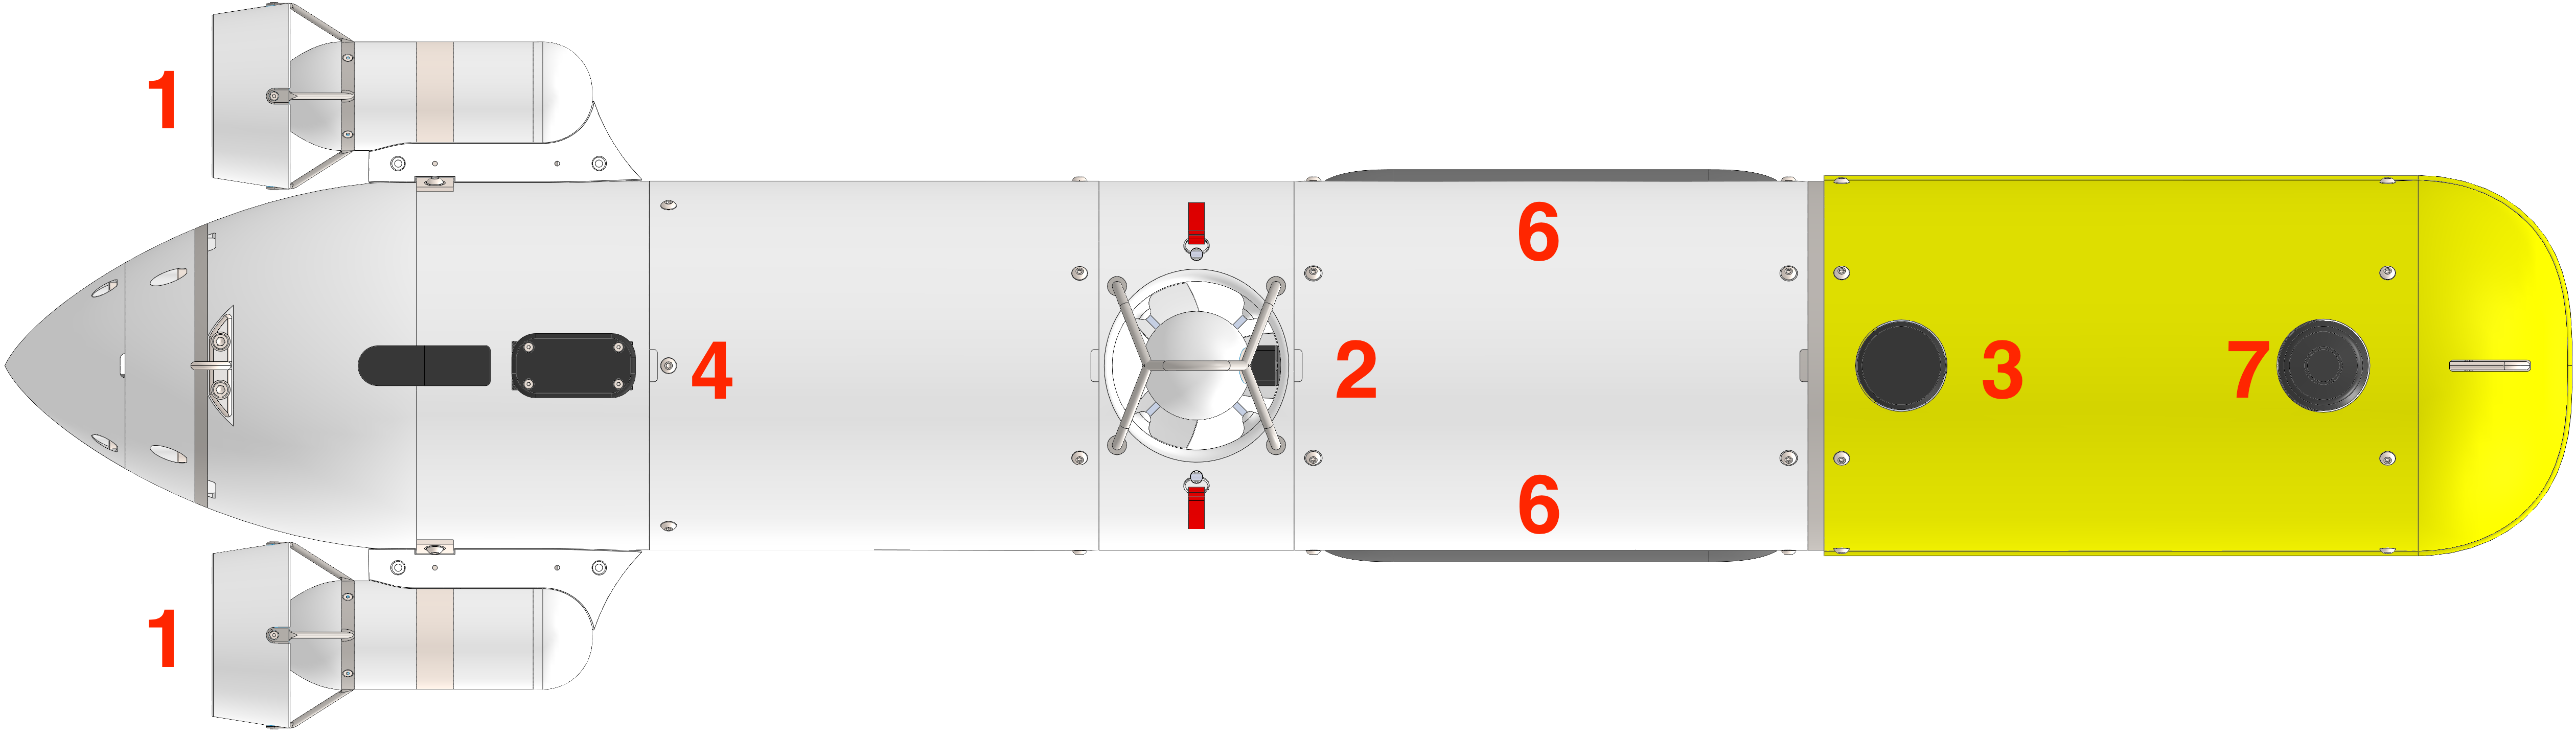
\includegraphics[width=.65\linewidth]{Sparus2FullTop}} \\%\quad
    \subfloat[Bottom view]
    {\label{fig:Sparus2FullBottom}%
     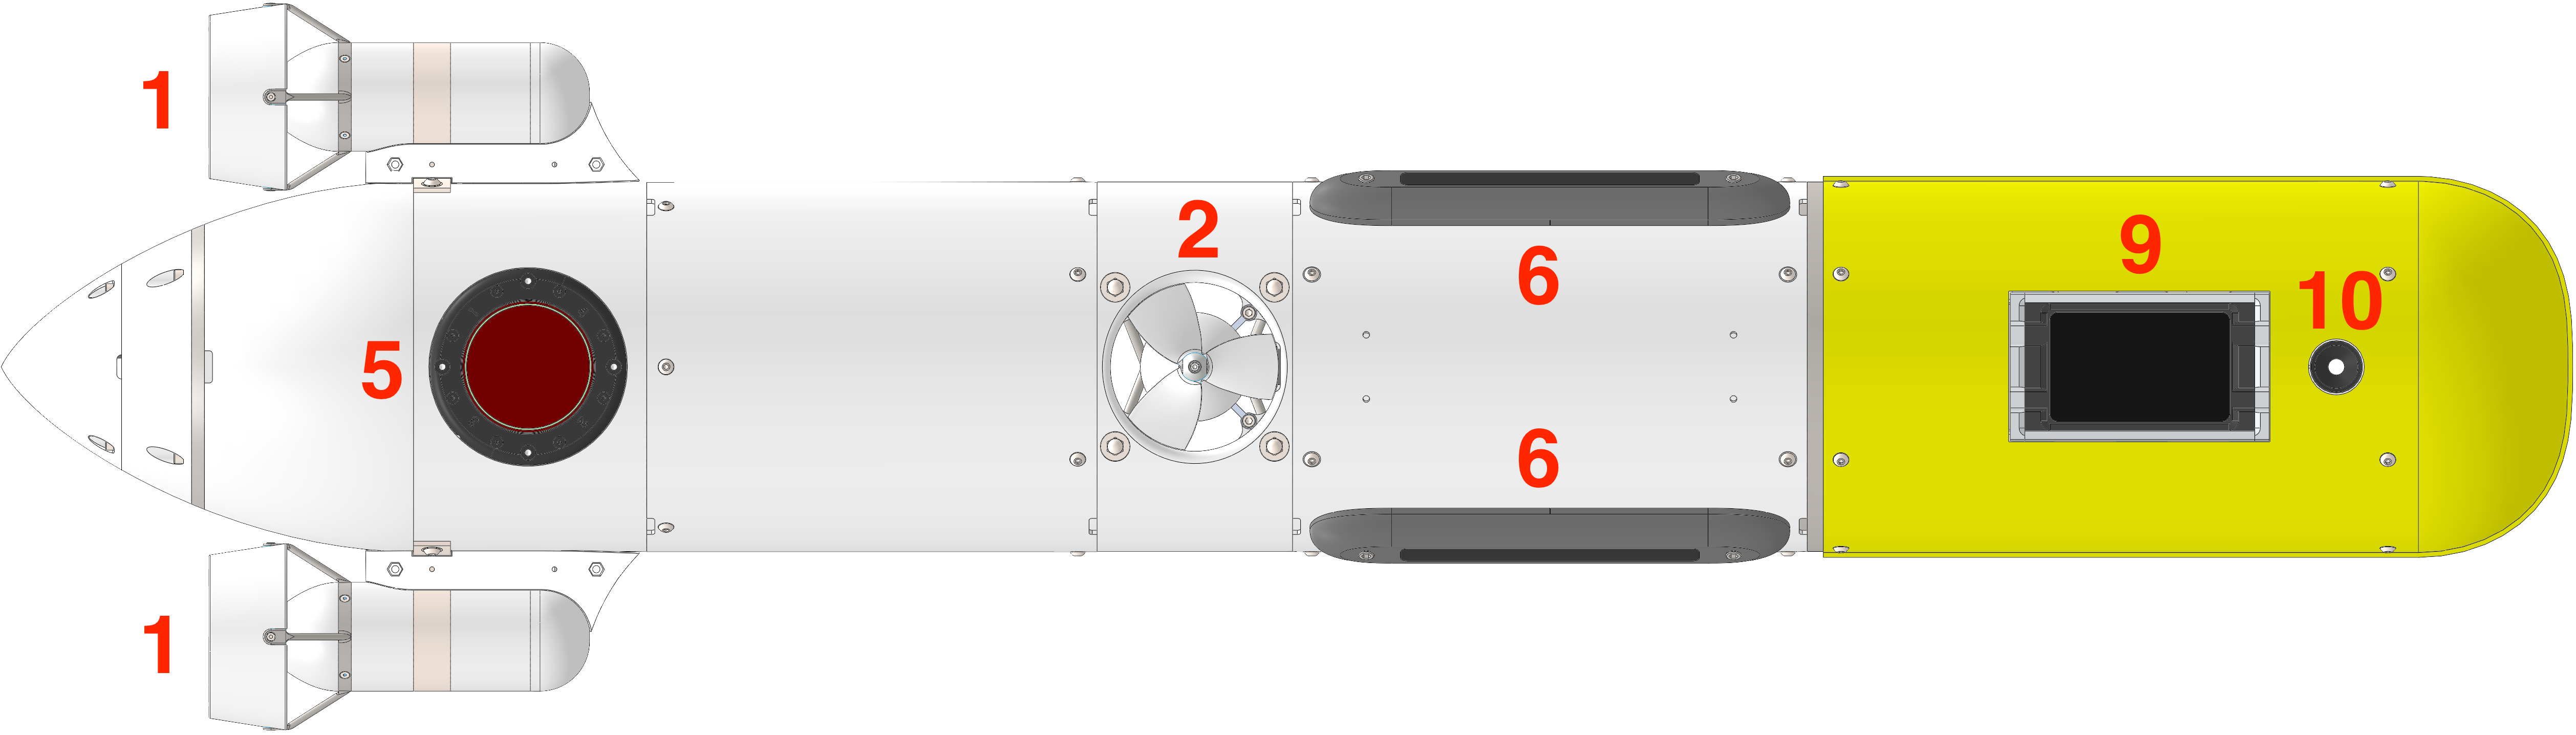
\includegraphics[width=.65\linewidth]{Sparus2FullBottom}}\\
    \subfloat[Lateral view]
    {\label{fig:Sparus2FullLateral}
    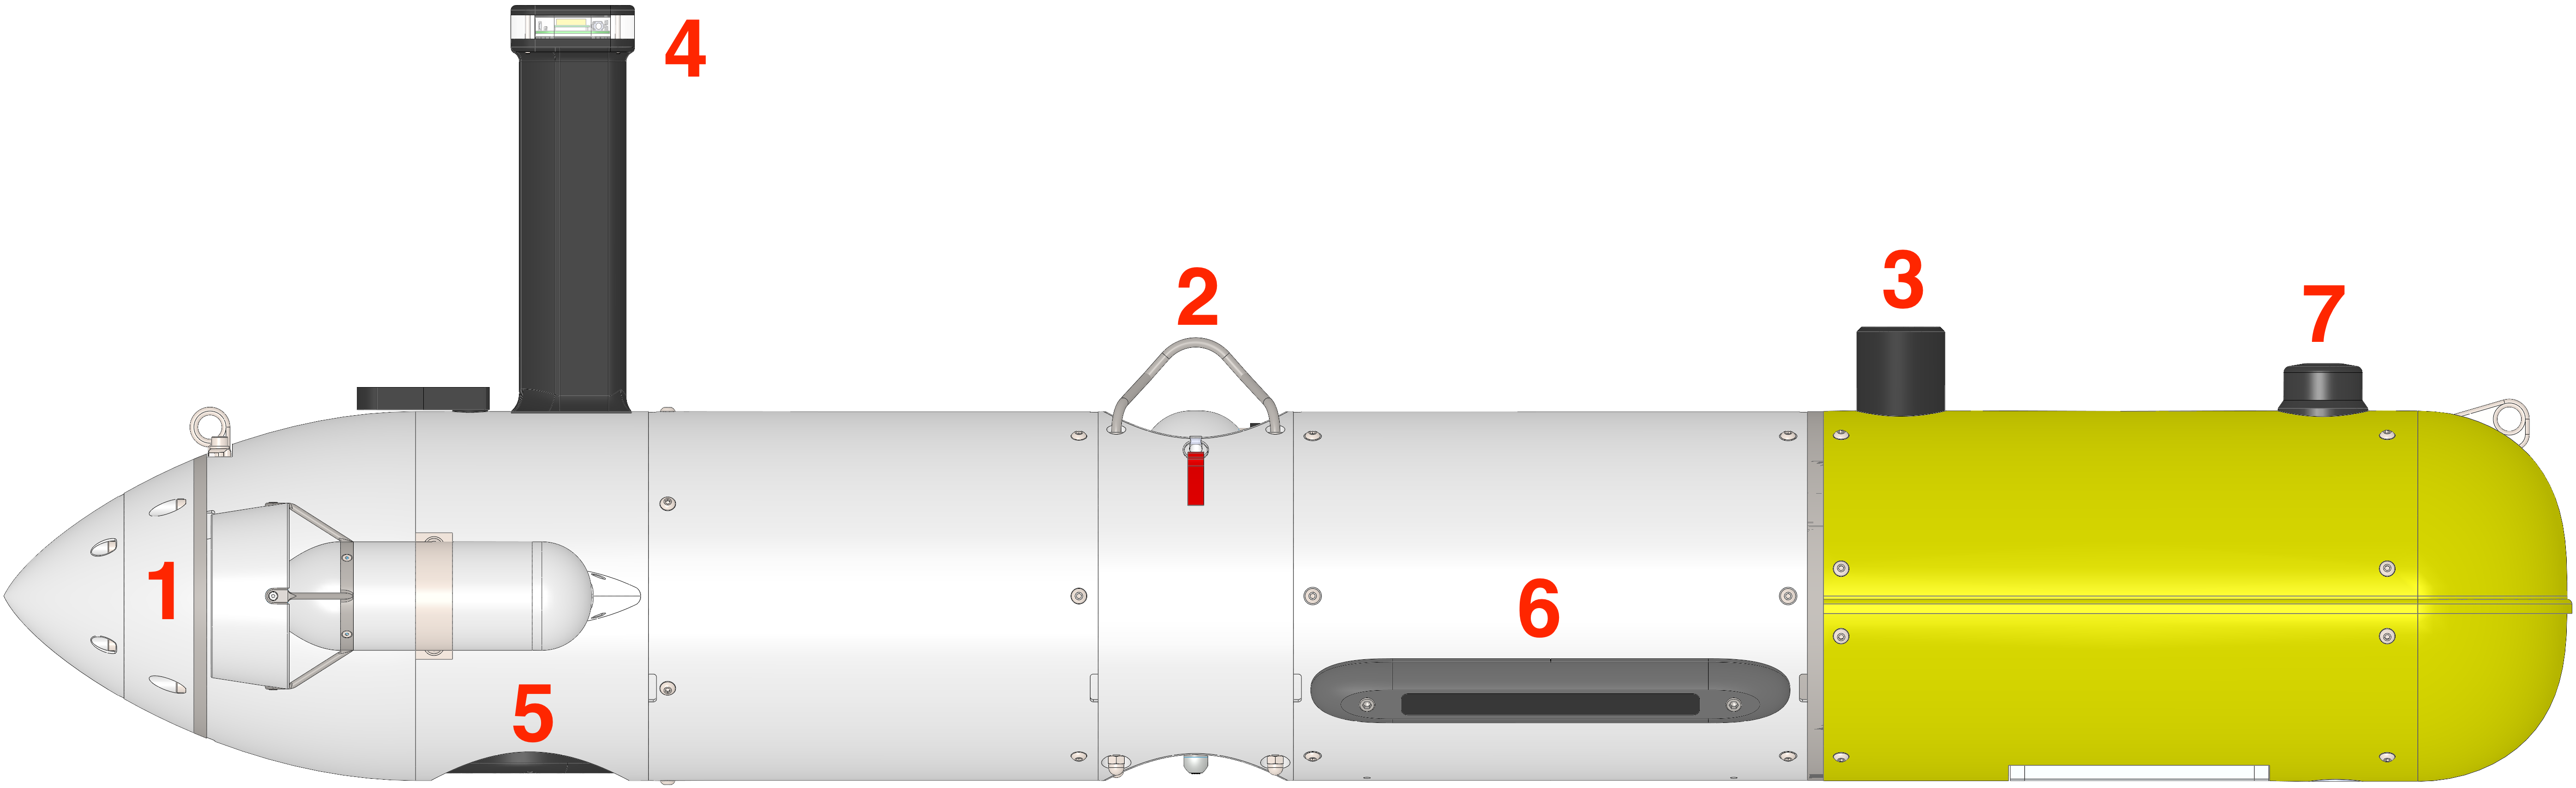
\includegraphics[width=.65\linewidth]{Sparus2FullLateral}}\\ %\quad
    \subfloat[3D view]
    {\label{fig:Sparus2Full3D}%
     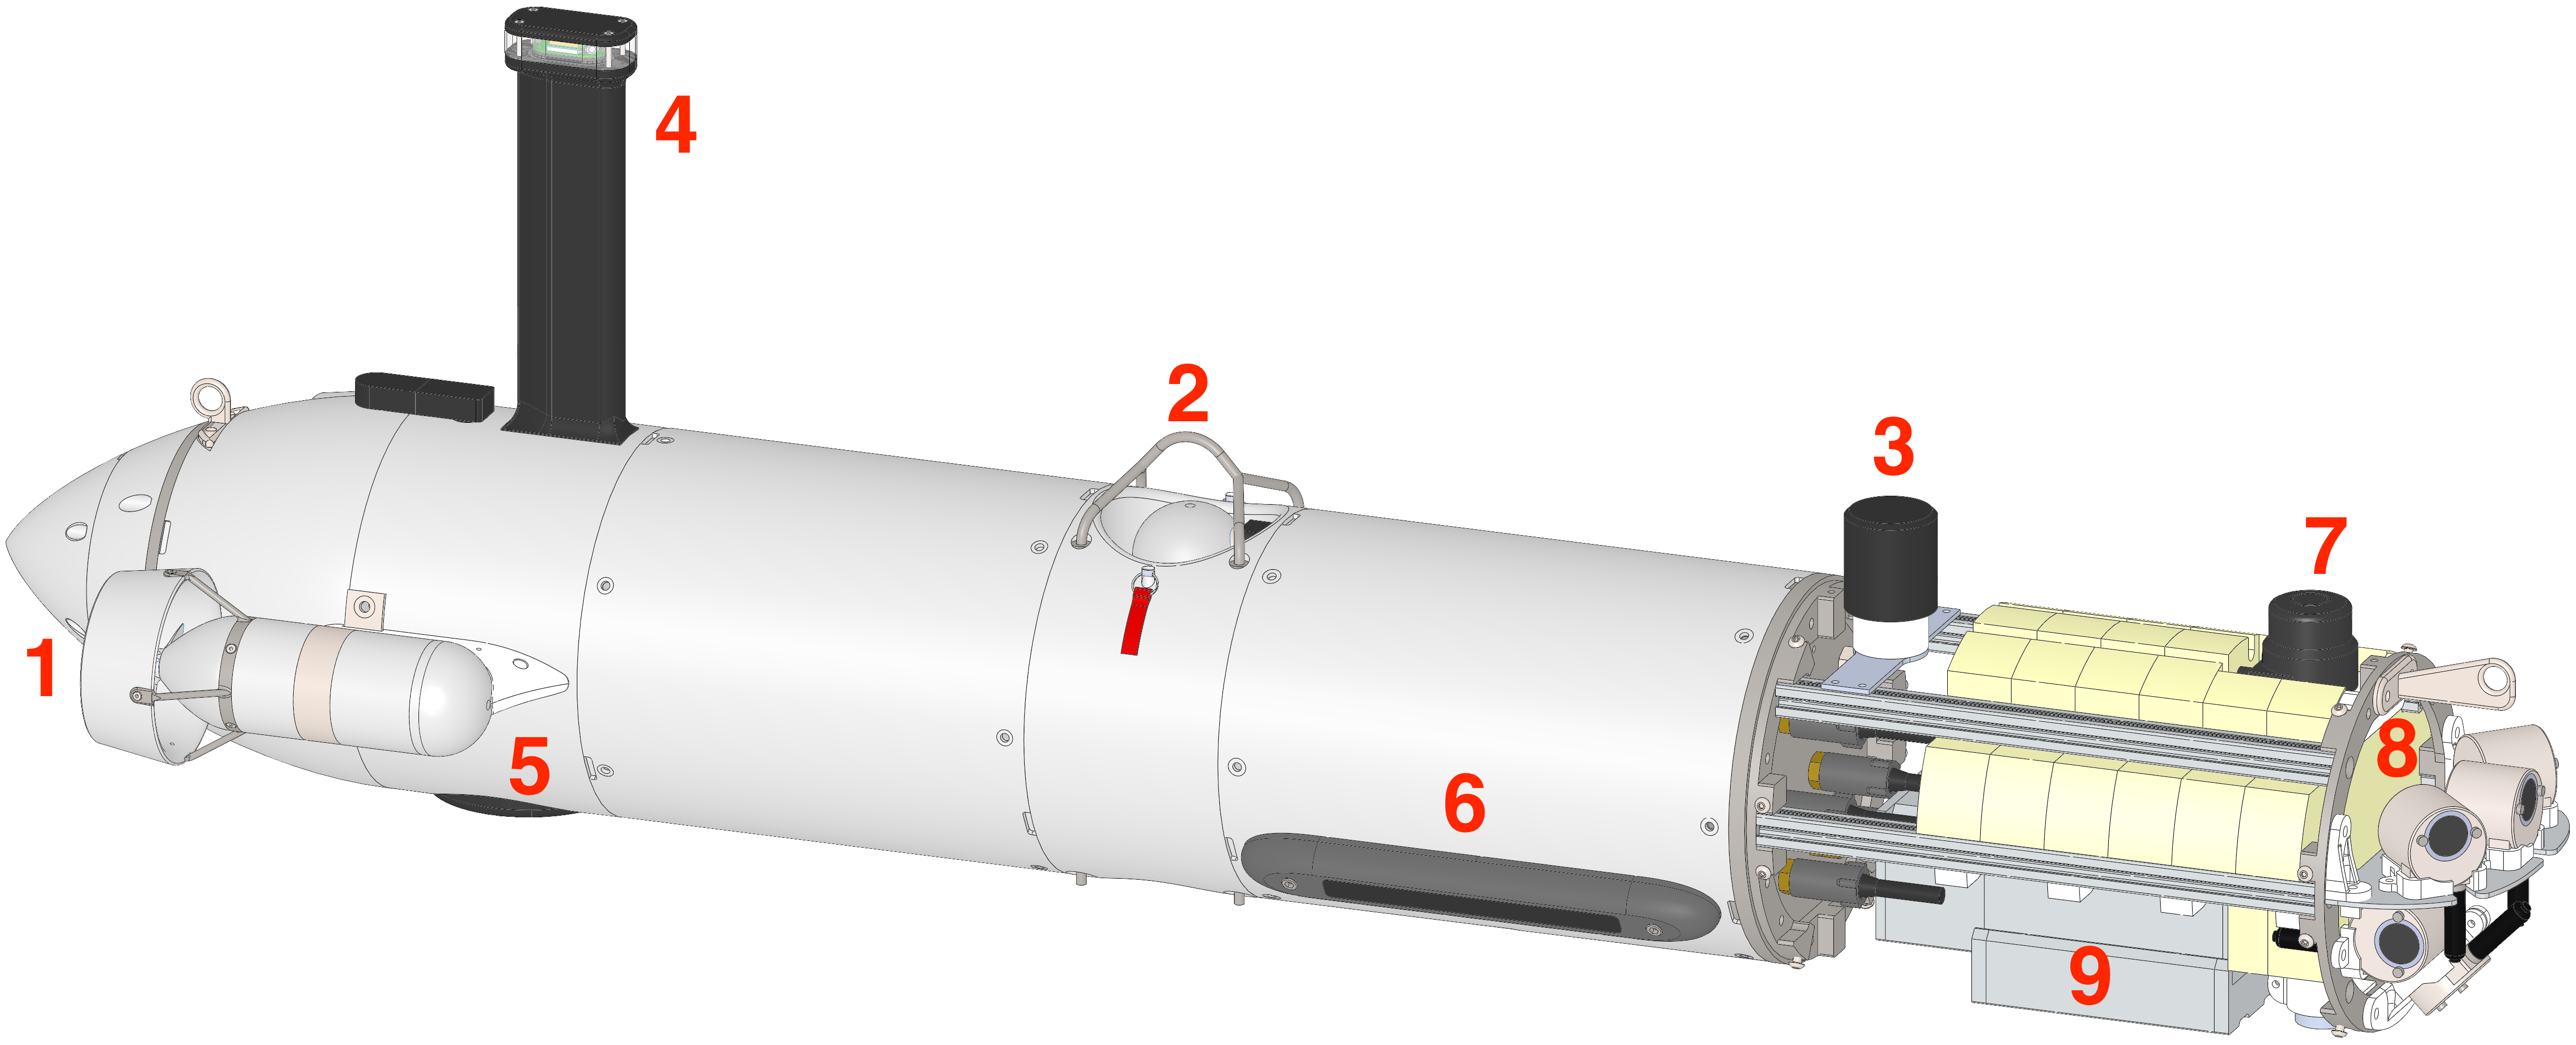
\includegraphics[width=.65\linewidth]{Sparus2Full3D}}
    \caption[Sparus~II AUV: top, bottom, lateral and 3D views, and its hardware
    elements.] 
    {Sparus~II AUV: top, bottom, lateral and 3D views. Different hardware parts
    can be observed, including the thrusters (1,2), the acoustic modem (3), the
    Wi-Fi and GPS (4), as well as interoceptive and exteroceptive sensors such
    as the DVL (5), side-scan sonar (6), mechanically-scanning imaging sonar
    (7), single-beam echosounders (8), multibeam sonar (9), and an optical
    camera (10).}
    \label{fig:Sparus2FullViews}
\end{figure}

In what software concerns, the Sparus~II \ac{AUV} is controlled through the
\acf{COLA2}~\cite{Palomeras2012}, which is a control architecture that is
completely integrated with the \acf{ROS}. Besides operating aboard real robots,
\ac{COLA2} can interact with the \acf{UWSim}~\cite{Prats2012}, which can import
\ac{3D} environment models and simulate the vehicle's sensors and dynamics with
high fidelity. Furthermore, the use of \ac{ROS} allows to easily integrate third
party tools, such as the \acf{OMPL} that offers a convenient framework that can
be adapted to specific path/motion planning problems~\cite{Sucan2012}.

% \begin{figure}[htbp]
% 	\centering
% 	\includegraphics[width=.85\linewidth]{MicronAperture} 
% 	\caption{\hl{Micron} Aperture.}
% 	\label{fig:MicronAperture}
% \end{figure}

\section{AsterX AUV}

The AsterX is a torpedo-shaped \ac{AUV} from the \acf{Ifremer}. This vehicle is
based on the Explorer~3000 \ac{AUV}, which is built by \ac{ISE}, from Canada.
The vehicle is rated for depths up to $3000 m$, and is equipped with one back
propulsion motor, three aft steering planes, and two fore planes. Similarly as
the Sparus~II, AsterX is equipped with a navigation sensor suite that includes a
pressure sensor, a \ac{DVL}, an \ac{IMU} and a GPS to receive position fixes
while at surface. It also has an acoustic modem, and a Wi-Fi antenna. This
\ac{AUV} also includes a modular payload area in the front, which may carry
different sensors, \eg a multibeam sonar. Figure~\ref{fig:AsterXFullViews}
depicts the AsterX \ac{AUV} at sea surface, and a schematic with its main inner
hardware devices distribution.

\begin{figure}[htbp]
    \myfloatalign
    \subfloat[AsterX \ac{AUV} at sea surface during in-water trials]
    {\label{fig:AsterXFullReal}%
     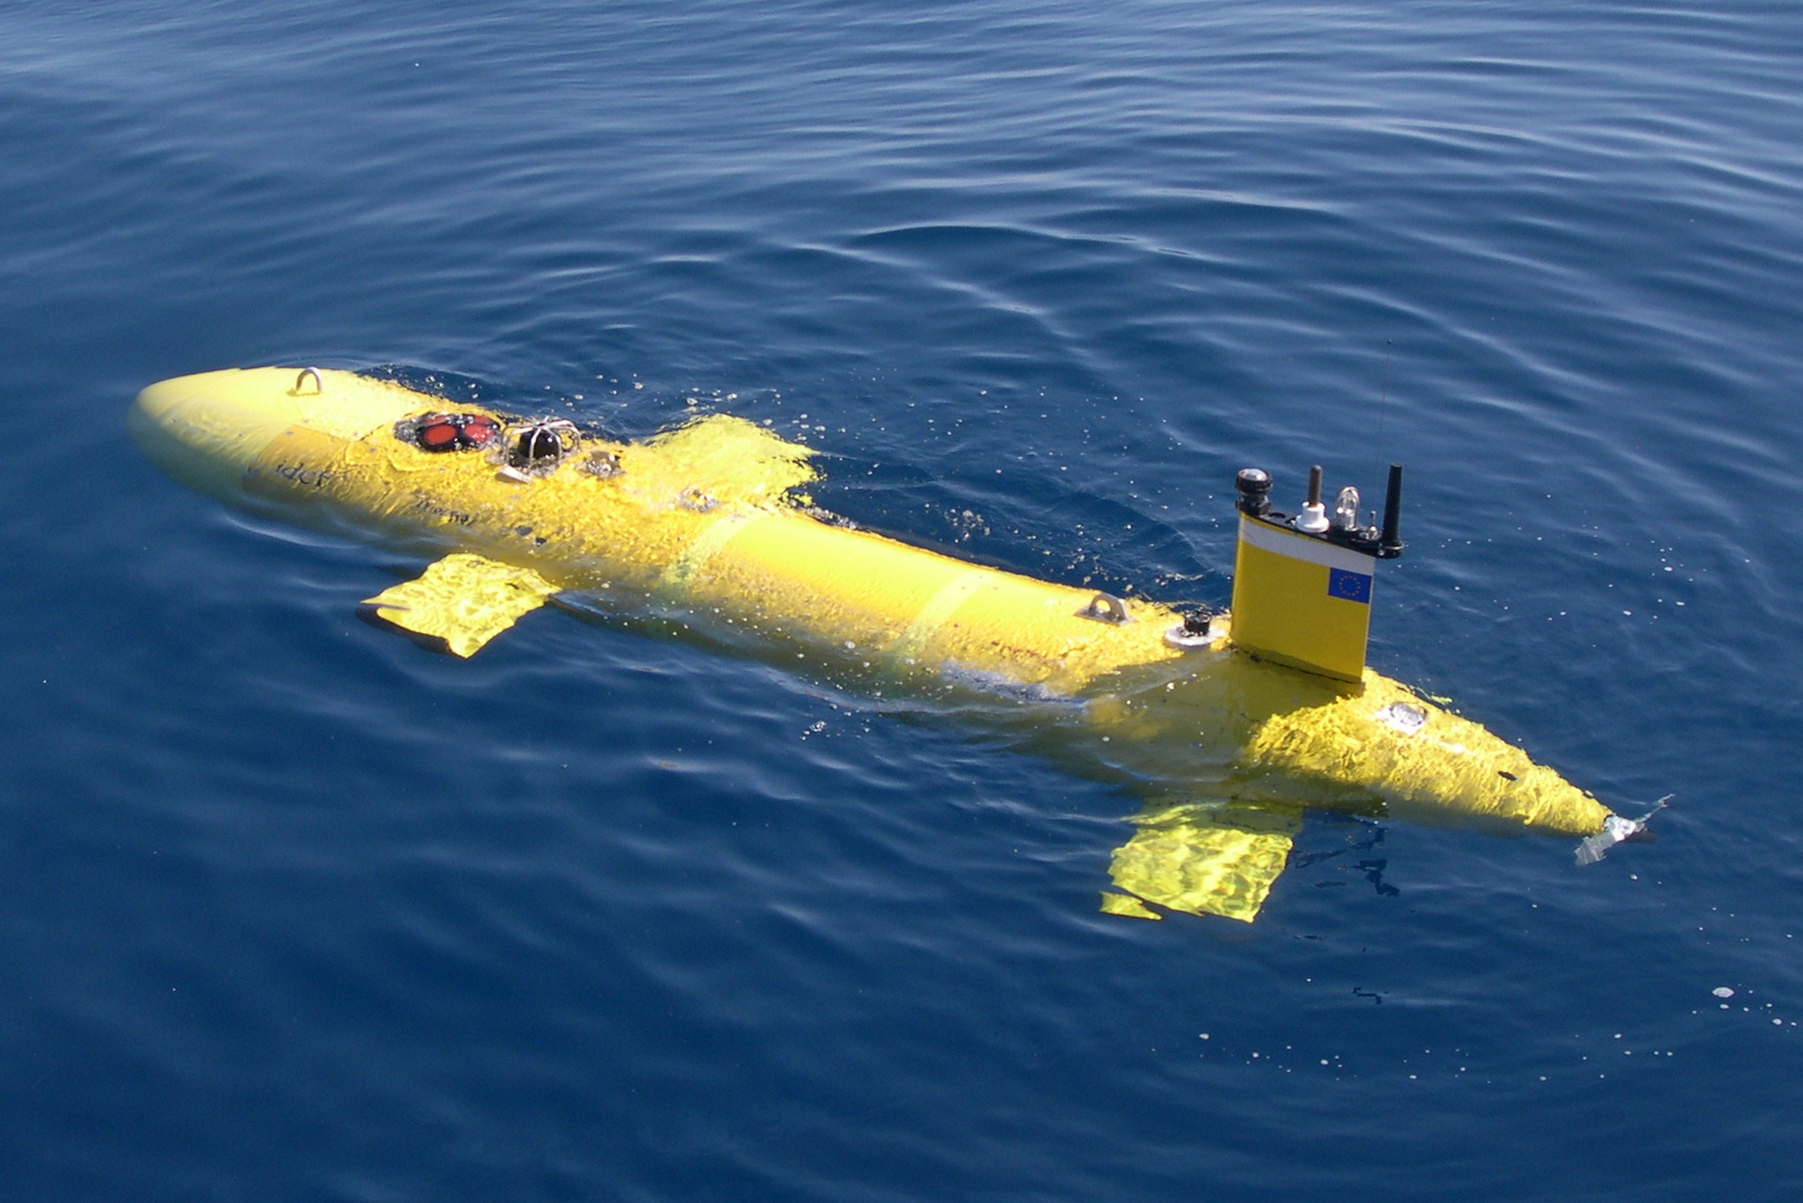
\includegraphics[width=.65\linewidth]{AsterXFullReal}}\\
%     \subfloat[Top view]
%     {\label{fig:AsterXFullTop}
%     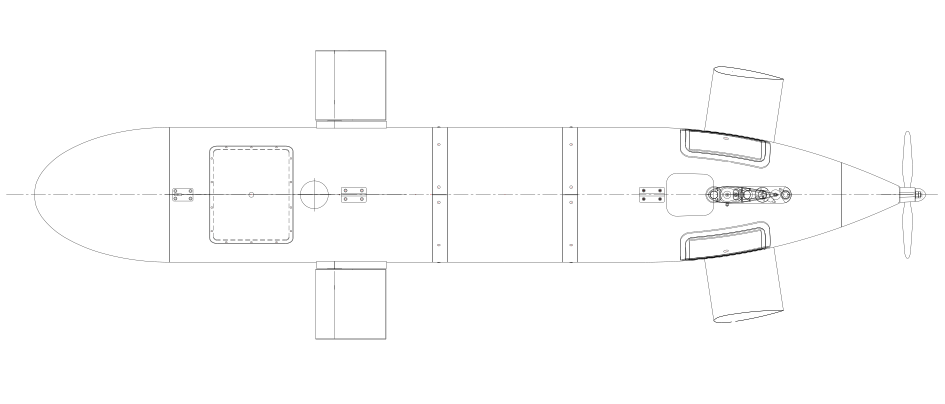
\includegraphics[width=.65\linewidth]{AsterXFullTop}} \\%\quad
    \subfloat[Lateral view]
    {\label{fig:AsterXFullLateral}
    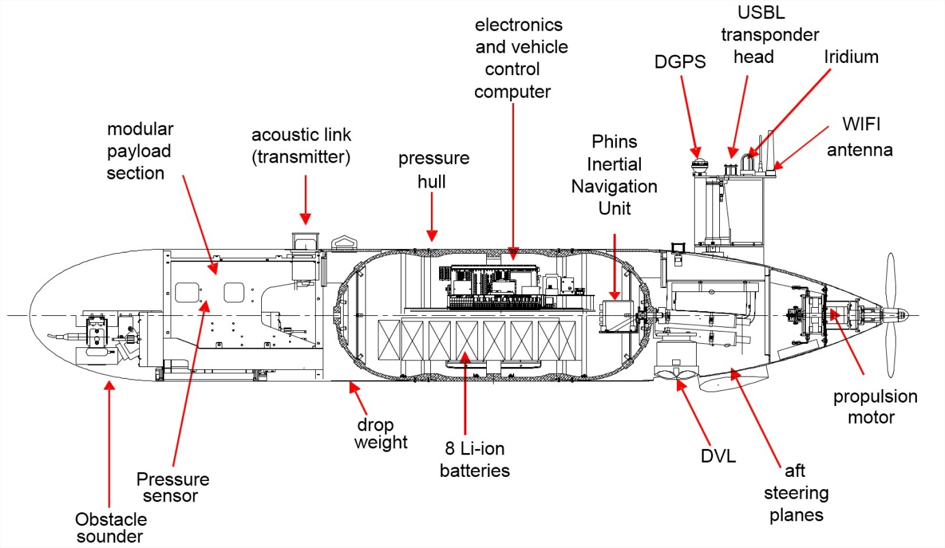
\includegraphics[width=.65\linewidth]{AsterXFullLateral}}\\ %\quad
    \caption[AsterX AUV at sea surface and its lateral view with a description of the
    different hardware elements.]
    {AsterX AUV at sea surface and its lateral view with a description of the
    different hardware elements.}
    \label{fig:AsterXFullViews}
\end{figure}

On the other hand, the AsterX's software architecture is composed of
three main functional blocks (see Fig.~\ref{fig:HighLevelControArch}).  Firstly,
the \ac{AUV} low-level controller, also referred as \textit{frontseat}, guides
the vehicle using the \ac{ACE} middleware. This controller is executed over QNX
operating system, thus guaranteeing real-time computation constraints.
Furthermore, this functional block also handles the vehicle's navigation and
safety routines. Secondly, the \textit{backseat} controller extends the
vehicle's capabilities and applications by easing the implementation of
high-level routines, such as algorithms for path/motion planning, path-tracking,
and docking. These routines can directly send low-level control setpoints. This
functional block has its own dedicated computer that works under the \ac{ROS}
(over Linux). Finally, the \textit{payload} controller acts as a bidirectional
interface between the interoceptive and exteroceptive sensors, and, on the other
hand, both the \textit{frontseat} and \textit{backseat} controllers.

\begin{figure}[htbp] %  figure placement: here, top, bottom, or page
\centering
	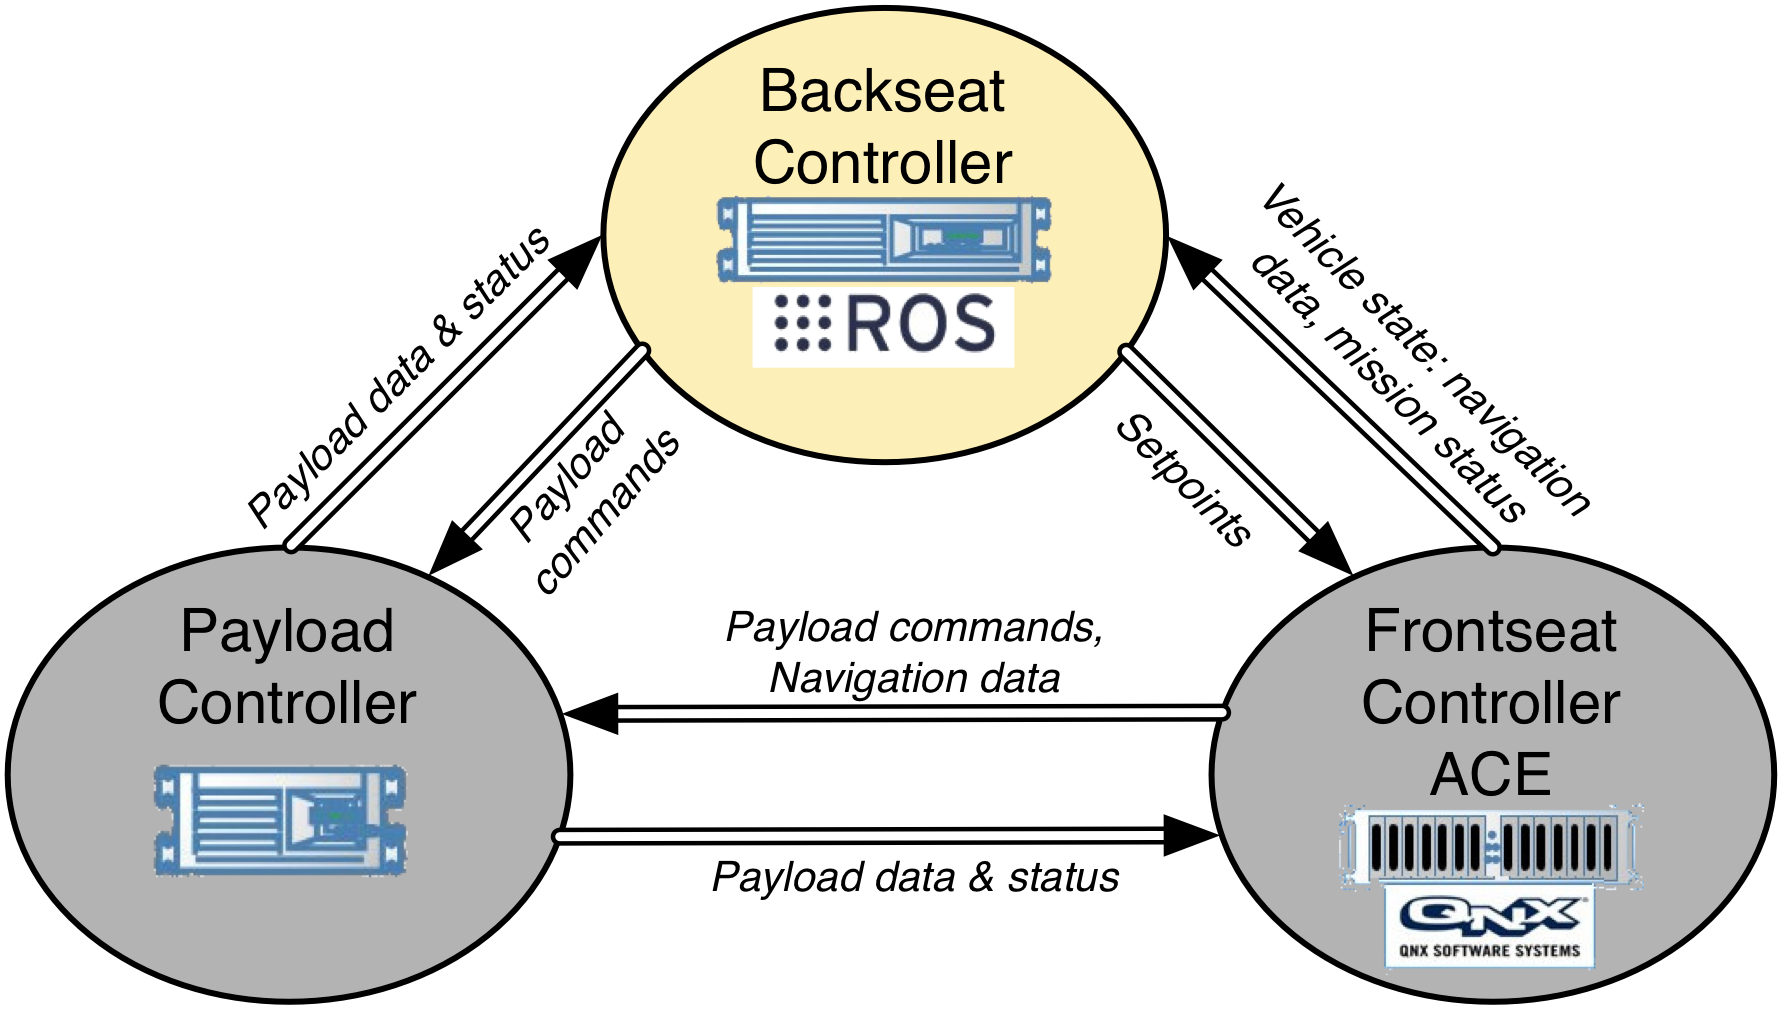
\includegraphics[width=.7\linewidth]{AsterX-Software-Architecture}
\caption[AsterX AUV software architecture.]
{AsterX \ac{AUV} software architecture}
\label{fig:HighLevelControArch}
\end{figure}


%********************************************************************
% Other Stuff in the Back
%*******************************************************
\cleardoublepage%********************************************************************
% Bibliography
%*******************************************************
% work-around to have small caps also here in the headline
\manualmark
\markboth{\spacedlowsmallcaps{\bibname}}{\spacedlowsmallcaps{\bibname}} % work-around to have small caps also
%\phantomsection 
\refstepcounter{dummy}
\addtocontents{toc}{\protect\vspace{\beforebibskip}} % to have the bib a bit from the rest in the toc
\addcontentsline{toc}{chapter}{\tocEntry{\bibname}}
\label{app:bibliography}

\printbibliography
% \bibliographystyle{plain}
% \bibliography{PhDThesis}

% \printbibliography[title=Bibliography,nottype=online]
% \printbibliography[title=Webography,type=online]
%\cleardoublepage%*******************************************************
% Declaration
%*******************************************************
\refstepcounter{dummy}
\pdfbookmark[0]{CERTIFICAT DE DIRECCIO DE TESI}{Certificat de Direccio de Tesi}
\chapter*{Certificat de Direcció de Tesi}
\thispagestyle{empty}

Dr. Pere Vilà Talleda and Dr. Lluís Fàbrega Soler, del Departament 
d’Arqui-tectura i Tecnologia de Computadors de la Universitat de Girona,

\bigskip

DECLAREM:

\bigskip

\noindent Que el treball titulat \textit{Word-Metric-based Greedy Routing for Cayley Graphs}, que presenta \myName per a l’obtenció
del títol de doctor, ha estat realitzat sota la nostra direcció i que compleix els requisits
per poder optar a Menció Internacional.

\bigskip

I, perquè així consti i tingui els efectes oportuns, signem aquest
document.

\bigskip
 
\noindent\textit{Girona, Juliol 2018}

\smallskip

\begin{flushright}
    \begin{tabular}{m{5cm} m{1.5cm} m{5cm}}
        \\ \cline{1-1} \cline{3-3}
        \centering\mySupervisor& &\centering\myOtherSupervisor \\
    \end{tabular}
\end{flushright}

%\cleardoublepage\pagestyle{empty}

\hfill

\vfill


\pdfbookmark[0]{Colophon}{colophon}
\section*{Colophon}
This document was typeset using the typographical look-and-feel \texttt{classicthesis} developed by Andr\'e Miede. 
The style was inspired by Robert Bringhurst's seminal book on typography ``\emph{The Elements of Typographic Style}''. 
\texttt{classicthesis} is available for both \LaTeX\ and \mLyX: 
\begin{center}
\url{https://bitbucket.org/amiede/classicthesis/}
\end{center}
Happy users of \texttt{classicthesis} usually send a real postcard to the author, a collection of postcards received so far is featured here: 
\begin{center}
\url{http://postcards.miede.de/}
\end{center}
 
\bigskip

\noindent\finalVersionString

%Hermann Zapf's \emph{Palatino} and \emph{Euler} type faces (Type~1 PostScript fonts \emph{URW
%Palladio L} and \emph{FPL}) are used. The ``typewriter'' text is typeset in \emph{Bera Mono}, 
%originally developed by Bitstream, Inc. as ``Bitstream Vera''. (Type~1 PostScript fonts were made 
%available by Malte Rosenau and
%Ulrich Dirr.)

%\paragraph{note:} The custom size of the textblock was calculated
%using the directions given by Mr. Bringhurst (pages 26--29 and
%175/176). 10~pt Palatino needs  133.21~pt for the string
%``abcdefghijklmnopqrstuvwxyz''. This yields a good line length between
%24--26~pc (288--312~pt). Using a ``\emph{double square textblock}''
%with a 1:2 ratio this results in a textblock of 312:624~pt (which
%includes the headline in this design). A good alternative would be the
%``\emph{golden section textblock}'' with a ratio of 1:1.62, here
%312:505.44~pt. For comparison, \texttt{DIV9} of the \texttt{typearea}
%package results in a line length of 389~pt (32.4~pc), which is by far
%too long. However, this information will only be of interest for
%hardcore pseudo-typographers like me.%
%
%To make your own calculations, use the following commands and look up
%the corresponding lengths in the book:
%\begin{verbatim}
%    \settowidth{\abcd}{abcdefghijklmnopqrstuvwxyz}
%    \the\abcd\ % prints the value of the length
%\end{verbatim}
%Please see the file \texttt{classicthesis.sty} for some precalculated 
%values for Palatino and Minion.
%
%    \settowidth{\abcd}{abcdefghijklmnopqrstuvwxyz}
%    \the\abcd\ % prints the value of the length





%********************************************************************
% Game Over: Restore, Restart, or Quit?
%*******************************************************
\end{document}
% ********************************************************************